% Options for packages loaded elsewhere
\PassOptionsToPackage{unicode}{hyperref}
\PassOptionsToPackage{hyphens}{url}
\PassOptionsToPackage{dvipsnames,svgnames,x11names}{xcolor}
%
\documentclass[
  letterpaper,
  DIV=11,
  numbers=noendperiod]{scrartcl}

\usepackage{amsmath,amssymb}
\usepackage{iftex}
\ifPDFTeX
  \usepackage[T1]{fontenc}
  \usepackage[utf8]{inputenc}
  \usepackage{textcomp} % provide euro and other symbols
\else % if luatex or xetex
  \usepackage{unicode-math}
  \defaultfontfeatures{Scale=MatchLowercase}
  \defaultfontfeatures[\rmfamily]{Ligatures=TeX,Scale=1}
\fi
\usepackage{lmodern}
\ifPDFTeX\else  
    % xetex/luatex font selection
\fi
% Use upquote if available, for straight quotes in verbatim environments
\IfFileExists{upquote.sty}{\usepackage{upquote}}{}
\IfFileExists{microtype.sty}{% use microtype if available
  \usepackage[]{microtype}
  \UseMicrotypeSet[protrusion]{basicmath} % disable protrusion for tt fonts
}{}
\makeatletter
\@ifundefined{KOMAClassName}{% if non-KOMA class
  \IfFileExists{parskip.sty}{%
    \usepackage{parskip}
  }{% else
    \setlength{\parindent}{0pt}
    \setlength{\parskip}{6pt plus 2pt minus 1pt}}
}{% if KOMA class
  \KOMAoptions{parskip=half}}
\makeatother
\usepackage{xcolor}
\setlength{\emergencystretch}{3em} % prevent overfull lines
\setcounter{secnumdepth}{-\maxdimen} % remove section numbering
% Make \paragraph and \subparagraph free-standing
\makeatletter
\ifx\paragraph\undefined\else
  \let\oldparagraph\paragraph
  \renewcommand{\paragraph}{
    \@ifstar
      \xxxParagraphStar
      \xxxParagraphNoStar
  }
  \newcommand{\xxxParagraphStar}[1]{\oldparagraph*{#1}\mbox{}}
  \newcommand{\xxxParagraphNoStar}[1]{\oldparagraph{#1}\mbox{}}
\fi
\ifx\subparagraph\undefined\else
  \let\oldsubparagraph\subparagraph
  \renewcommand{\subparagraph}{
    \@ifstar
      \xxxSubParagraphStar
      \xxxSubParagraphNoStar
  }
  \newcommand{\xxxSubParagraphStar}[1]{\oldsubparagraph*{#1}\mbox{}}
  \newcommand{\xxxSubParagraphNoStar}[1]{\oldsubparagraph{#1}\mbox{}}
\fi
\makeatother

\usepackage{color}
\usepackage{fancyvrb}
\newcommand{\VerbBar}{|}
\newcommand{\VERB}{\Verb[commandchars=\\\{\}]}
\DefineVerbatimEnvironment{Highlighting}{Verbatim}{commandchars=\\\{\}}
% Add ',fontsize=\small' for more characters per line
\usepackage{framed}
\definecolor{shadecolor}{RGB}{241,243,245}
\newenvironment{Shaded}{\begin{snugshade}}{\end{snugshade}}
\newcommand{\AlertTok}[1]{\textcolor[rgb]{0.68,0.00,0.00}{#1}}
\newcommand{\AnnotationTok}[1]{\textcolor[rgb]{0.37,0.37,0.37}{#1}}
\newcommand{\AttributeTok}[1]{\textcolor[rgb]{0.40,0.45,0.13}{#1}}
\newcommand{\BaseNTok}[1]{\textcolor[rgb]{0.68,0.00,0.00}{#1}}
\newcommand{\BuiltInTok}[1]{\textcolor[rgb]{0.00,0.23,0.31}{#1}}
\newcommand{\CharTok}[1]{\textcolor[rgb]{0.13,0.47,0.30}{#1}}
\newcommand{\CommentTok}[1]{\textcolor[rgb]{0.37,0.37,0.37}{#1}}
\newcommand{\CommentVarTok}[1]{\textcolor[rgb]{0.37,0.37,0.37}{\textit{#1}}}
\newcommand{\ConstantTok}[1]{\textcolor[rgb]{0.56,0.35,0.01}{#1}}
\newcommand{\ControlFlowTok}[1]{\textcolor[rgb]{0.00,0.23,0.31}{\textbf{#1}}}
\newcommand{\DataTypeTok}[1]{\textcolor[rgb]{0.68,0.00,0.00}{#1}}
\newcommand{\DecValTok}[1]{\textcolor[rgb]{0.68,0.00,0.00}{#1}}
\newcommand{\DocumentationTok}[1]{\textcolor[rgb]{0.37,0.37,0.37}{\textit{#1}}}
\newcommand{\ErrorTok}[1]{\textcolor[rgb]{0.68,0.00,0.00}{#1}}
\newcommand{\ExtensionTok}[1]{\textcolor[rgb]{0.00,0.23,0.31}{#1}}
\newcommand{\FloatTok}[1]{\textcolor[rgb]{0.68,0.00,0.00}{#1}}
\newcommand{\FunctionTok}[1]{\textcolor[rgb]{0.28,0.35,0.67}{#1}}
\newcommand{\ImportTok}[1]{\textcolor[rgb]{0.00,0.46,0.62}{#1}}
\newcommand{\InformationTok}[1]{\textcolor[rgb]{0.37,0.37,0.37}{#1}}
\newcommand{\KeywordTok}[1]{\textcolor[rgb]{0.00,0.23,0.31}{\textbf{#1}}}
\newcommand{\NormalTok}[1]{\textcolor[rgb]{0.00,0.23,0.31}{#1}}
\newcommand{\OperatorTok}[1]{\textcolor[rgb]{0.37,0.37,0.37}{#1}}
\newcommand{\OtherTok}[1]{\textcolor[rgb]{0.00,0.23,0.31}{#1}}
\newcommand{\PreprocessorTok}[1]{\textcolor[rgb]{0.68,0.00,0.00}{#1}}
\newcommand{\RegionMarkerTok}[1]{\textcolor[rgb]{0.00,0.23,0.31}{#1}}
\newcommand{\SpecialCharTok}[1]{\textcolor[rgb]{0.37,0.37,0.37}{#1}}
\newcommand{\SpecialStringTok}[1]{\textcolor[rgb]{0.13,0.47,0.30}{#1}}
\newcommand{\StringTok}[1]{\textcolor[rgb]{0.13,0.47,0.30}{#1}}
\newcommand{\VariableTok}[1]{\textcolor[rgb]{0.07,0.07,0.07}{#1}}
\newcommand{\VerbatimStringTok}[1]{\textcolor[rgb]{0.13,0.47,0.30}{#1}}
\newcommand{\WarningTok}[1]{\textcolor[rgb]{0.37,0.37,0.37}{\textit{#1}}}

\providecommand{\tightlist}{%
  \setlength{\itemsep}{0pt}\setlength{\parskip}{0pt}}\usepackage{longtable,booktabs,array}
\usepackage{calc} % for calculating minipage widths
% Correct order of tables after \paragraph or \subparagraph
\usepackage{etoolbox}
\makeatletter
\patchcmd\longtable{\par}{\if@noskipsec\mbox{}\fi\par}{}{}
\makeatother
% Allow footnotes in longtable head/foot
\IfFileExists{footnotehyper.sty}{\usepackage{footnotehyper}}{\usepackage{footnote}}
\makesavenoteenv{longtable}
\usepackage{graphicx}
\makeatletter
\def\maxwidth{\ifdim\Gin@nat@width>\linewidth\linewidth\else\Gin@nat@width\fi}
\def\maxheight{\ifdim\Gin@nat@height>\textheight\textheight\else\Gin@nat@height\fi}
\makeatother
% Scale images if necessary, so that they will not overflow the page
% margins by default, and it is still possible to overwrite the defaults
% using explicit options in \includegraphics[width, height, ...]{}
\setkeys{Gin}{width=\maxwidth,height=\maxheight,keepaspectratio}
% Set default figure placement to htbp
\makeatletter
\def\fps@figure{htbp}
\makeatother
% definitions for citeproc citations
\NewDocumentCommand\citeproctext{}{}
\NewDocumentCommand\citeproc{mm}{%
  \begingroup\def\citeproctext{#2}\cite{#1}\endgroup}
\makeatletter
 % allow citations to break across lines
 \let\@cite@ofmt\@firstofone
 % avoid brackets around text for \cite:
 \def\@biblabel#1{}
 \def\@cite#1#2{{#1\if@tempswa , #2\fi}}
\makeatother
\newlength{\cslhangindent}
\setlength{\cslhangindent}{1.5em}
\newlength{\csllabelwidth}
\setlength{\csllabelwidth}{3em}
\newenvironment{CSLReferences}[2] % #1 hanging-indent, #2 entry-spacing
 {\begin{list}{}{%
  \setlength{\itemindent}{0pt}
  \setlength{\leftmargin}{0pt}
  \setlength{\parsep}{0pt}
  % turn on hanging indent if param 1 is 1
  \ifodd #1
   \setlength{\leftmargin}{\cslhangindent}
   \setlength{\itemindent}{-1\cslhangindent}
  \fi
  % set entry spacing
  \setlength{\itemsep}{#2\baselineskip}}}
 {\end{list}}
\usepackage{calc}
\newcommand{\CSLBlock}[1]{\hfill\break\parbox[t]{\linewidth}{\strut\ignorespaces#1\strut}}
\newcommand{\CSLLeftMargin}[1]{\parbox[t]{\csllabelwidth}{\strut#1\strut}}
\newcommand{\CSLRightInline}[1]{\parbox[t]{\linewidth - \csllabelwidth}{\strut#1\strut}}
\newcommand{\CSLIndent}[1]{\hspace{\cslhangindent}#1}

\KOMAoption{captions}{tableheading}
\makeatletter
\@ifpackageloaded{caption}{}{\usepackage{caption}}
\AtBeginDocument{%
\ifdefined\contentsname
  \renewcommand*\contentsname{Table of contents}
\else
  \newcommand\contentsname{Table of contents}
\fi
\ifdefined\listfigurename
  \renewcommand*\listfigurename{List of Figures}
\else
  \newcommand\listfigurename{List of Figures}
\fi
\ifdefined\listtablename
  \renewcommand*\listtablename{List of Tables}
\else
  \newcommand\listtablename{List of Tables}
\fi
\ifdefined\figurename
  \renewcommand*\figurename{Figure}
\else
  \newcommand\figurename{Figure}
\fi
\ifdefined\tablename
  \renewcommand*\tablename{Table}
\else
  \newcommand\tablename{Table}
\fi
}
\@ifpackageloaded{float}{}{\usepackage{float}}
\floatstyle{ruled}
\@ifundefined{c@chapter}{\newfloat{codelisting}{h}{lop}}{\newfloat{codelisting}{h}{lop}[chapter]}
\floatname{codelisting}{Listing}
\newcommand*\listoflistings{\listof{codelisting}{List of Listings}}
\makeatother
\makeatletter
\makeatother
\makeatletter
\@ifpackageloaded{caption}{}{\usepackage{caption}}
\@ifpackageloaded{subcaption}{}{\usepackage{subcaption}}
\makeatother

\ifLuaTeX
  \usepackage{selnolig}  % disable illegal ligatures
\fi
\usepackage{bookmark}

\IfFileExists{xurl.sty}{\usepackage{xurl}}{} % add URL line breaks if available
\urlstyle{same} % disable monospaced font for URLs
\hypersetup{
  pdftitle={NPS Scraper - Full Code},
  colorlinks=true,
  linkcolor={blue},
  filecolor={Maroon},
  citecolor={Blue},
  urlcolor={Blue},
  pdfcreator={LaTeX via pandoc}}


\title{NPS Scraper - Full Code}
\usepackage{etoolbox}
\makeatletter
\providecommand{\subtitle}[1]{% add subtitle to \maketitle
  \apptocmd{\@title}{\par {\large #1 \par}}{}{}
}
\makeatother
\subtitle{DSAN 5500: Data Structures, Objects, and Algorithms in Python}
\author{Gentry Lamb}
\date{}

\begin{document}
\maketitle


\subsection{Abstract}\label{abstract}

This project presents the design and implementation of an ETL (Extract,
Transform, Load) pipeline built to automate collecting, processing, and
delivering timely insights from the National Park Service (NPS) API.
Motivated by personal experiences planning trips across 21 national
parks, the project addresses a persistent challenge for outdoor
enthusiasts: fragmented, inconsistent access to critical park
information such as closures, alerts, and available activities. While
the NPS API offers structured access to this data, it remains difficult
to use effectively without a more accessible interface or automation.

The developed solution leverages the Python-based orchestration tool
Prefect to manage tasks and flows, ensuring that data pipelines run
reliably and can be scheduled for recurring updates. Raw data from the
NPS API is extracted across three key domains (parks, alerts, and
activities) and then validated using Pydantic to ensure consistency and
data quality. Alerts are further enriched through sentiment analysis and
a custom severity scoring system, enabling travelers to filter and
prioritize alerts based on urgency. The resulting structured datasets
are saved in \texttt{.jsonl} format for easy reuse, analysis, and
visualization.

A key deliverable is a weekly Markdown report summarizing the most
relevant alerts and changes, along with an interactive map to visualize
national park status. While this implementation is focused on a Minimum
Viable Product (MVP), it provides a scalable foundation for future
enhancements such as real-time alerting, itinerary planning, or
personalized recommendations. This project demonstrates how automated
data pipelines can bridge the gap between raw API data and actionable
insights for end users, using modern tools in Python to improve
decision-making and trip planning for outdoor adventurers and public
land users.

\subsection{Motivation}\label{motivation}

Known for its natural beauty and vast wilderness, Montana is home to two
of the most iconic national parks in the United States. Growing up in
this awe-inspiring state instilled a deep appreciation for nature and a
lifelong commitment to spending time outdoors. After moving to Colorado
for college, that commitment evolved into a personal goal: to complete a
backpacking trip in every U.S. national park. I have completed 21 thus
far, exactly one-third of the current federally designated sites.
Planning those trips has become as much a part of the experience as the
trails themselves. Balancing routes, permits, weather forecasts, and
increasingly, real-time alerts about fire danger, road closures, and
other unexpected events is a large part of making these trips a reality.

That planning process is often frustrating at times. Information is
scattered across park-specific websites, not always up to date, and hard
to monitor consistently. I found myself checking the National Park
Service (NPS) websites over and over before a trip, just to make sure I
hadn't missed a sudden trail closure or hazardous condition. That's when
I discovered the NPS API (\citeproc{ref-nps_api}{2017}), which makes
structured data on park alerts, activities, and general park info
accessible through a RESTful interface. It felt like the missing link,
raw access to the exact data I needed, but with none of the
user-friendly polish to make it practical for regular use.

This project grew out of a desire to fill that gap. I wanted to build
something that didn't just pull park data for its own sake, but that
could help travelers like me make informed decisions. With that goal, I
designed an ETL (Extract, Transform, Load) pipeline in Python that could
automatically turn information on park websites into usable insights for
travelers and planners. This project not only fulfills a personal goal -
to create a better tool for planning future trips to national parks -
but also serves as a testbed for applying best practices in pipeline
design, including orchestration, scheduling, data validation, and
artifact generation. The system is built to be extensible, too. Future
iterations could include personalized park filters, travel-ready
itineraries, or real-time notifications. For now, the core functionality
offers something simple but impactful: regular and reliable insight into
the changing conditions across our national parks.

\subsection{Problem Statement}\label{problem-statement}

As mentioned above, the current method for gathering information on
national parks, such as alerts and activity availability, is largely
manual. Users must visit multiple NPS web pages individually to get
up-to-date information. While the National Park Service (NPS) API offers
structured access to data on alerts, activities, and park information,
the data can be difficult to understand in its raw form. It lacks a
user-friendly interface and doesn't solve the core problem of timely,
consolidated delivery. That's where an ETL pipeline can help. By
automating the collection, transformation, and distribution of this
information, the pipeline reduces manual effort and creates a more
reliable, centralized source of truth.

There were a myriad of ideas I wanted to implement in this project, but
given the time constraints of the semester, I had to narrow in on a
Minimum Viable Product (MVP). The MVP focuses on using
\href{https://www.prefect.io/}{Prefect}, a Python-based workflow
orchestration tool, to create a pipeline that extracts data from the NPS
API, validates it with
\href{https://docs.pydantic.dev/latest/}{Pydantic}, transforms it into
traveler-relevant summaries, and loads it to a database so that it can
be used later. The pipeline is scheduled to execute weekly, producing
two main deliverables: a Markdown report summarizing the various
suggestions and an interactive map showing the most recent park alerts.
This MVP addresses the core workflow inefficiencies while providing a
strong foundation for future expansion.

\subsection{Extract, Transform, Load (ETL)
Pipeline}\label{extract-transform-load-etl-pipeline}

The core of this project implements a robust and automated ETL pipeline
that collects, cleans, enriches, and stores data from the National Park
Service API. The goal of this pipeline is to take raw, unprocessed data
about sites owned by the NPS and turn it into meaningful, organized, and
ready-to-use information for further analysis or reporting. This process
is automated using \href{https://www.prefect.io/}{Prefect}, which helps
break the workflow into smaller, manageable tasks that can be monitored,
run on a schedule, and easily extended in the future.

\subsubsection{Extract - Gathering the
Data}\label{extract---gathering-the-data}

A key strength of this pipeline lies in its ability to consistently
extract, clean, and validate three interconnected datasets from the NPS
API. These datasets include parks, alerts, and activities. Each of these
serves a distinct purpose but are designed to integrate smoothly into a
unified data pipeline.

The parks dataset provides foundational information about each site
managed by the NPS. This includes the park's name, park code, location
(including state and geographic coordinates), a short descriptive
overview, its designation (such as ``National Park,'' ``Historic Site,''
or ``National Seashore.''), and various other features. This dataset
anchors the pipeline, supplying the essential context for any mapping,
alert monitoring, or activity planning feature built downstream.

The alerts dataset was the primary focus initially as I wanted to gather
data that changed significantly day-to-day. It includes time-sensitive
messages issued by the NPS to communicate urgent or important updates
about park conditions. These messages range from weather closures and
fire warnings to temporary restrictions, safety tips, and general
updates on services or amenities. The content is often unstructured and
highly variable in tone and detail. Because of this variability,
additional downstream processing is applied later in the pipeline to
assess each alert's sentiment and severity.

Finally, the activities dataset catalogs the range of recreational and
educational opportunities available across the park system. Activities
can include hiking, camping, boating, wildlife viewing, ranger-led
tours, and more. Each entry links one or more activities to specific
parks, forming a crucial bridge between park information and user
preferences.

Once these datasets are extracted from the API, they undergo a
structured data validation process. Rather than loading the raw data
directly into spreadsheets or data frames, this pipeline uses a more
robust and maintainable approach by defining formal data models using
Pydantic, a Python library that enforces data types and rules. For each
dataset, a dedicated class is defined. These classes lay out the
expected fields, their required formats (such as strings, floats, or
lists), and any default values to use when information is missing or
malformed. This validation layer serves as a powerful early-warning
system. For example, if a park's location data is missing or incorrectly
formatted, the model catches it immediately and either supplies a
default value or safely omits the record, depending on the use case.
Similarly, if an alert is missing a description or an activity is
assigned an invalid name, these issues are surfaced and handled during
validation, not later when they might cause errors in analysis.

\subsubsection{Transform - Enriching the
Data}\label{transform---enriching-the-data}

While all three datasets are cleaned and formatted, the alerts dataset
is given special attention because it's the most dynamic and
unstructured. These alerts often contain free-text descriptions that
vary widely in tone, importance, and length. To make them more useful,
the pipeline performs two key transformations.

\paragraph{Sentiment Analysis}\label{sentiment-analysis}

The pipeline evaluates the emotional tone of each alert using a tool
that measures sentiment. This helps identify whether an alert is
neutral, negative (e.g., a warning or danger), or slightly positive by
assigning a value between negative 1 and positive 1. For example, an
alert that says ``Caution: Recent bear sightings'' would register as
more negative than something like ``Information: Parking lot
construction.'' This helps quantify how urgent or concerning an alert
might feel to a visitor.

\paragraph{Severity Scoring}\label{severity-scoring}

Each alert also comes with a predefined category assigned by the NPS,
such as ``Information,'' ``Caution,'' ``Park Closure,'' or ``Danger.''
These categories are mapped to severity scores based on how serious they
are. For instance, a ``Park Closure'' or ``Danger'' alert is scored
higher than a general ``Information'' alert. While there is no
definitive answer for how severe an alert is, I use values in the range
of 1-5 as a basis.

\paragraph{Final Score}\label{final-score}

To make alerts easier to sort and prioritize, the pipeline combines the
sentiment and severity into a single composite score. This final score
provides a way to rank alerts in terms of overall urgency and
importance, taking into account both what the alert says and how it's
likely to affect visitors. This enrichment process transforms plain text
into something that can be compared, filtered, and visualized. This
makes it far more useful than the raw descriptions alone.

\subsubsection{Load - Saving the
Outputs}\label{load---saving-the-outputs}

Once all data is cleaned, validated, and transformed, it is saved into
structured files (in \texttt{.jsonl} format). These files serve as the
project's internal ``database'' and are well-organized, easy to read,
and compatible with many tools for analysis or reporting. Each of the
three datasets (parks, alerts, and activities) are saved separately.
This modular approach allows different parts of the data to be reused or
analyzed independently depending on the needs of the application. Early
in the project, there was consideration of using a more traditional
database system, such as MongoDB for flexible document storage or SQL
for structured relational queries. However, given the relatively modest
size of the datasets and the timeline constraints of the project, it
became clear that implementing a full database was not necessary at this
stage. Instead, the decision to use \texttt{.jsonl} files prioritized
transparency and simplicity. This approach enabled faster iteration and
easier debugging, while still leaving open the possibility of scaling up
to a database-backed architecture later.

\subsection{Automation with Prefect}\label{automation-with-prefect}

To ensure that the entire pipeline, from data extraction to
transformation, validation, and final loading, runs in a reliable and
repeatable way, I used \href{https://www.prefect.io/}{Prefect}, as it
provides a clear and scalable way to define workflows using two key
building blocks: \texttt{tasks} and \texttt{flows}. Each key operation
in the ETL process is defined as a \texttt{task} in Prefect. For
example:

\begin{itemize}
\tightlist
\item
  The \texttt{get\_parks()} task queries API to gather information about
  parks.
\item
  The \texttt{transform\_alerts()} task takes validated alerts, adding
  information on alert sentiment, severity, and score.
\item
  The \texttt{load\_into\_db()} task handles serialization and saving of
  the final cleaned data to disk.
\end{itemize}

These tasks are then composed into \texttt{flows}, higher-level
processes that determine the order and logic of task execution. For
instance, the main \texttt{scrape\_NPS()} flow coordinates the full
process of extracting, validating, and saving data for all three
datasets: parks, alerts, and activities. Prefect handles this
orchestration automatically, so that tasks are executed in the proper
sequence and only rerun when necessary.

\begin{figure}[H]

{\centering 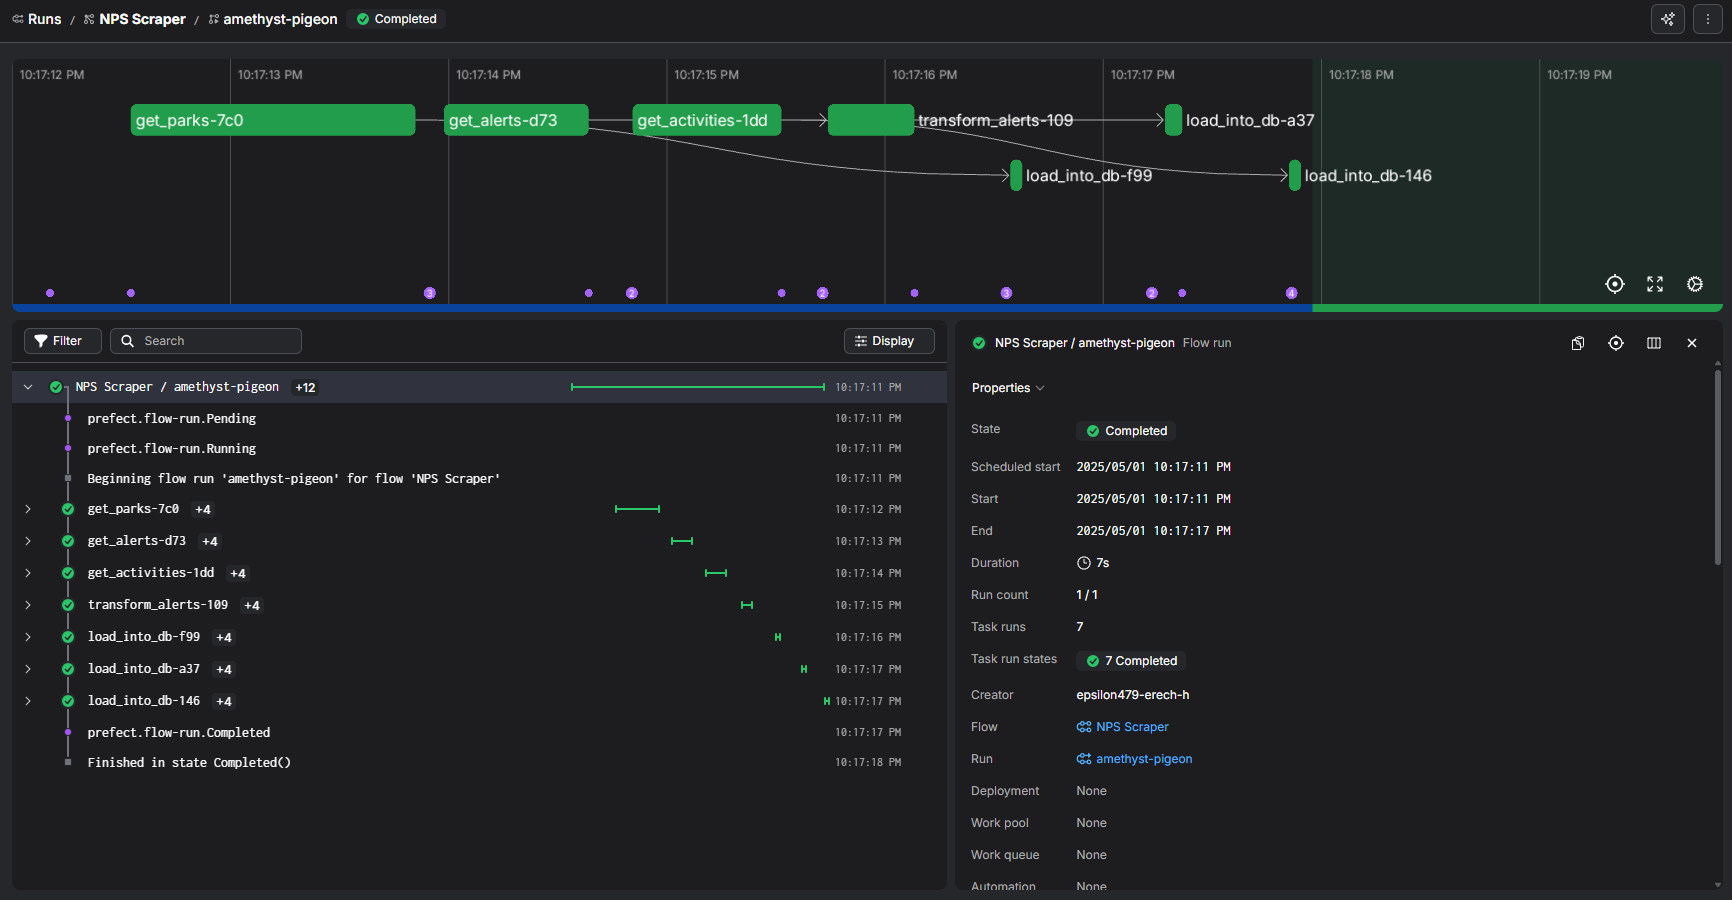
\includegraphics{assets/nps-scraper-flow.png}

}

\caption{Example Run Output of NPS Scraper in Prefect}

\end{figure}%

Using Prefect provided several key benefits that helped shape the
success and maintainability of the pipeline. It enabled easy automation,
allowing flows to be scheduled for regular execution, such as weekly
updates, without the need for manual triggers. Further, Prefect's
built-in user interface offered robust monitoring and logging
capabilities. Each task's status could be tracked in real-time, and logs
were automatically generated, making it easy to catch and debug issues
like failed downloads or other discrepancies. With each task defined
independently, new functionality could be introduced with minimal
disruption to the existing flow. Beyond these benefits, Prefect also
made development more flexible and less error-prone. I was able to
experiment with and test tasks in isolation before integrating them into
the full pipeline, which made debugging more straightforward and helped
ensure that each component worked correctly on its own. This modular and
organized approach significantly enhanced the clarity and reliability of
the overall project.

\subsection{Artifacts and Useful
Output}\label{artifacts-and-useful-output}

Beyond processing and saving structured data, the pipeline also produces
two final artifacts. These user-facing outputs represent the culmination
of the ETL process and its real-world utility. To generate these
artifacts, a second Prefect flow was created specifically for the
reporting and visualization steps. Each artifact highlights a different
aspect of the data and serves a distinct purpose for end users. An
example run of this flow from the Prefect UI is shown below.

\begin{figure}[H]

{\centering 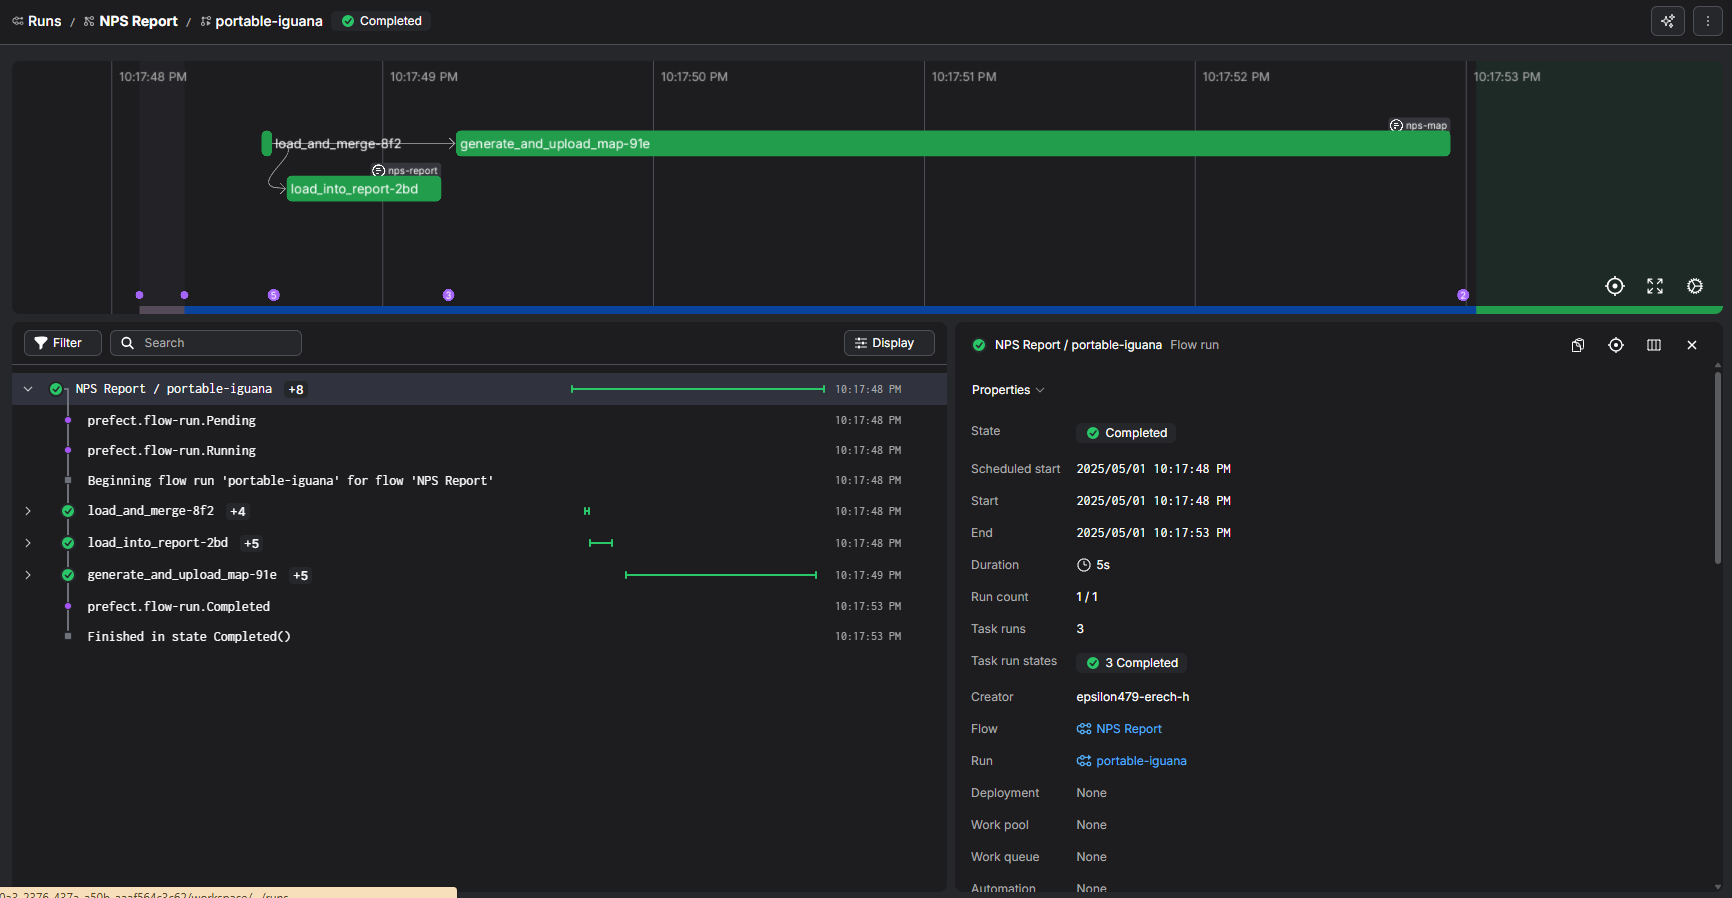
\includegraphics{assets/nps-report-flow.png}

}

\caption{Example Run Output of NPS Report in Prefect}

\end{figure}%

\subsubsection{Markdown Report}\label{markdown-report}

The first artifact is a generated Markdown report, built by pulling
insights from the processed park and alert data. This report includes
several key summaries and visual highlights: the total number of alerts
across all parks, a breakdown of the most common alert types, and a
ranked list of parks experiencing the highest number of active alerts.
It also includes detailed tables showing parks ranked on different
metrics, with direct links to the park pages. Behind the scenes,
generating this report required substantial data transformation like
grouping, filtering, and summarizing. Functions like
\texttt{aggregate\_data()} and \texttt{get\_top\_sites()} were developed
to handle these transformations cleanly and consistently. The final
report is written to markdown using a custom function and is designed to
be portable. It can be embedded directly into a website, emailed as part
of a weekly digest, or converted into HTML or PDF for broader
distribution. Since it is regenerated automatically whenever the
pipeline runs, it provides accurate updates about conditions across the
National Park system, without requiring manual reporting or analysis.
Below is an example of this report.

\section{NPS Scraping Report}\label{nps-scraping-report}

\textbf{Report Date:} 02-May-2025

\textbf{Total Alerts Collected:} 645

\textbf{Site Type:} National Park or Preserve

\subsection{⚠️ Most Common Alert Types}\label{most-common-alert-types}

The most frequently occurring alert types were:

\begin{longtable}[]{@{}lr@{}}
\toprule\noalign{}
Category & Count \\
\midrule\noalign{}
\endhead
\bottomrule\noalign{}
\endlastfoot
Information & 327 \\
Park Closure & 182 \\
Caution & 122 \\
Danger & 14 \\
\end{longtable}

\subsection{❗ National Park or Preserve with the Most
Alerts}\label{national-park-or-preserve-with-the-most-alerts}

\begin{longtable}[]{@{}
  >{\raggedleft\arraybackslash}p{(\columnwidth - 12\tabcolsep) * \real{0.0288}}
  >{\raggedright\arraybackslash}p{(\columnwidth - 12\tabcolsep) * \real{0.2302}}
  >{\raggedright\arraybackslash}p{(\columnwidth - 12\tabcolsep) * \real{0.0863}}
  >{\raggedright\arraybackslash}p{(\columnwidth - 12\tabcolsep) * \real{0.2590}}
  >{\raggedleft\arraybackslash}p{(\columnwidth - 12\tabcolsep) * \real{0.1295}}
  >{\raggedleft\arraybackslash}p{(\columnwidth - 12\tabcolsep) * \real{0.1223}}
  >{\raggedleft\arraybackslash}p{(\columnwidth - 12\tabcolsep) * \real{0.1439}}@{}}
\toprule\noalign{}
\begin{minipage}[b]{\linewidth}\raggedleft
\end{minipage} & \begin{minipage}[b]{\linewidth}\raggedright
Site Name
\end{minipage} & \begin{minipage}[b]{\linewidth}\raggedright
State(s)
\end{minipage} & \begin{minipage}[b]{\linewidth}\raggedright
Site Website
\end{minipage} & \begin{minipage}[b]{\linewidth}\raggedleft
Avg. Sentiment
\end{minipage} & \begin{minipage}[b]{\linewidth}\raggedleft
Avg. Severity
\end{minipage} & \begin{minipage}[b]{\linewidth}\raggedleft
Number of Alerts
\end{minipage} \\
\midrule\noalign{}
\endhead
\bottomrule\noalign{}
\endlastfoot
1 & Everglades National Park & FL & https://www.nps.gov/ever/index.htm &
0.221978 & 1.72222 & 9 \\
2 & Shenandoah National Park & VA & https://www.nps.gov/shen/index.htm &
0.0252875 & 0.75 & 8 \\
3 & Cuyahoga Valley National Park & OH &
https://www.nps.gov/cuva/index.htm & 0.00995714 & 2 & 7 \\
4 & Carlsbad Caverns National Park & NM &
https://www.nps.gov/cave/index.htm & -0.164714 & 0.571429 & 7 \\
5 & North Cascades National Park & WA &
https://www.nps.gov/noca/index.htm & -0.0222 & 2.07143 & 7 \\
6 & Saguaro National Park & AZ & https://www.nps.gov/sagu/index.htm &
0.0896 & 0.8 & 5 \\
7 & Zion National Park & UT & https://www.nps.gov/zion/index.htm &
-0.19254 & 1.6 & 5 \\
8 & White Sands National Park & NM & https://www.nps.gov/whsa/index.htm
& 0.16462 & 1 & 5 \\
9 & Lassen Volcanic National Park & CA &
https://www.nps.gov/lavo/index.htm & -0.19908 & 1.7 & 5 \\
10 & Mount Rainier National Park & WA &
https://www.nps.gov/mora/index.htm & 0.02632 & 2.1 & 5 \\
\end{longtable}

\subsection{🚫 National Park or Preserve with Highest Alert
Scores}\label{national-park-or-preserve-with-highest-alert-scores}

Using a scoring system that adjusts for both alert type and sentiment,
we've identified the 10 sites currently facing the most serious issues:

\begin{longtable}[]{@{}
  >{\raggedleft\arraybackslash}p{(\columnwidth - 12\tabcolsep) * \real{0.0284}}
  >{\raggedright\arraybackslash}p{(\columnwidth - 12\tabcolsep) * \real{0.2766}}
  >{\raggedright\arraybackslash}p{(\columnwidth - 12\tabcolsep) * \real{0.0851}}
  >{\raggedright\arraybackslash}p{(\columnwidth - 12\tabcolsep) * \real{0.2553}}
  >{\raggedleft\arraybackslash}p{(\columnwidth - 12\tabcolsep) * \real{0.1277}}
  >{\raggedleft\arraybackslash}p{(\columnwidth - 12\tabcolsep) * \real{0.1206}}
  >{\raggedleft\arraybackslash}p{(\columnwidth - 12\tabcolsep) * \real{0.1064}}@{}}
\toprule\noalign{}
\begin{minipage}[b]{\linewidth}\raggedleft
\end{minipage} & \begin{minipage}[b]{\linewidth}\raggedright
Site Name
\end{minipage} & \begin{minipage}[b]{\linewidth}\raggedright
State(s)
\end{minipage} & \begin{minipage}[b]{\linewidth}\raggedright
Site Website
\end{minipage} & \begin{minipage}[b]{\linewidth}\raggedleft
Avg. Sentiment
\end{minipage} & \begin{minipage}[b]{\linewidth}\raggedleft
Avg. Severity
\end{minipage} & \begin{minipage}[b]{\linewidth}\raggedleft
Alert Score
\end{minipage} \\
\midrule\noalign{}
\endhead
\bottomrule\noalign{}
\endlastfoot
1 & North Cascades National Park & WA &
https://www.nps.gov/noca/index.htm & -0.0222 & 2.07143 & 100 \\
2 & Cuyahoga Valley National Park & OH &
https://www.nps.gov/cuva/index.htm & 0.00995714 & 2 & 96.17 \\
3 & Lassen Volcanic National Park & CA &
https://www.nps.gov/lavo/index.htm & -0.19908 & 1.7 & 79.2 \\
4 & Sequoia \& Kings Canyon National Parks & CA &
https://www.nps.gov/seki/index.htm & -0.305133 & 3 & 76.05 \\
5 & Guadalupe Mountains National Park & TX &
https://www.nps.gov/gumo/index.htm & -0.532367 & 2.16667 & 72.67 \\
6 & Everglades National Park & FL & https://www.nps.gov/ever/index.htm &
0.221978 & 1.72222 & 70.5 \\
7 & Hawaiʻi Volcanoes National Park & HI &
https://www.nps.gov/havo/index.htm & -0.07105 & 3 & 67.71 \\
8 & Zion National Park & UT & https://www.nps.gov/zion/index.htm &
-0.19254 & 1.6 & 66.62 \\
9 & Mount Rainier National Park & WA &
https://www.nps.gov/mora/index.htm & 0.02632 & 2.1 & 66.48 \\
10 & Mojave National Preserve & CA & https://www.nps.gov/moja/index.htm
& 0.0550333 & 3 & 60.83 \\
\end{longtable}

\subsection{✅ National Park or Preserve with Highest Alert
Scores}\label{national-park-or-preserve-with-highest-alert-scores-1}

Conversely, these 10 sites are currently facing the fewest and least
serious issues:

\begin{longtable}[]{@{}
  >{\raggedleft\arraybackslash}p{(\columnwidth - 12\tabcolsep) * \real{0.0270}}
  >{\raggedright\arraybackslash}p{(\columnwidth - 12\tabcolsep) * \real{0.3108}}
  >{\raggedright\arraybackslash}p{(\columnwidth - 12\tabcolsep) * \real{0.0811}}
  >{\raggedright\arraybackslash}p{(\columnwidth - 12\tabcolsep) * \real{0.2432}}
  >{\raggedleft\arraybackslash}p{(\columnwidth - 12\tabcolsep) * \real{0.1216}}
  >{\raggedleft\arraybackslash}p{(\columnwidth - 12\tabcolsep) * \real{0.1149}}
  >{\raggedleft\arraybackslash}p{(\columnwidth - 12\tabcolsep) * \real{0.1014}}@{}}
\toprule\noalign{}
\begin{minipage}[b]{\linewidth}\raggedleft
\end{minipage} & \begin{minipage}[b]{\linewidth}\raggedright
Site Name
\end{minipage} & \begin{minipage}[b]{\linewidth}\raggedright
State(s)
\end{minipage} & \begin{minipage}[b]{\linewidth}\raggedright
Site Website
\end{minipage} & \begin{minipage}[b]{\linewidth}\raggedleft
Avg. Sentiment
\end{minipage} & \begin{minipage}[b]{\linewidth}\raggedleft
Avg. Severity
\end{minipage} & \begin{minipage}[b]{\linewidth}\raggedleft
Alert Score
\end{minipage} \\
\midrule\noalign{}
\endhead
\bottomrule\noalign{}
\endlastfoot
1 & Gates Of The Arctic National Park \& Preserve & AK &
https://www.nps.gov/gaar/index.htm & 0.4767 & 0.5 & 0 \\
2 & Isle Royale National Park & MI & https://www.nps.gov/isro/index.htm
& 0.6597 & 1 & 0.52 \\
3 & Joshua Tree National Park & CA & https://www.nps.gov/jotr/index.htm
& 0.6249 & 1 & 0.75 \\
4 & Death Valley National Park & CA,NV &
https://www.nps.gov/deva/index.htm & 0.25 & 0.5 & 0.75 \\
5 & Great Sand Dunes National Park \& Preserve & CO &
https://www.nps.gov/grsa/index.htm & 0.6167 & 1 & 0.8 \\
6 & Valles Caldera National Preserve & NM &
https://www.nps.gov/vall/index.htm & 0.2263 & 0.5 & 0.83 \\
7 & Grand Teton National Park & WY & https://www.nps.gov/grte/index.htm
& 0.2263 & 0.5 & 0.83 \\
8 & Hot Springs National Park & AR & https://www.nps.gov/hosp/index.htm
& 0 & 0.5 & 1.58 \\
9 & New River Gorge National Park \& Preserve & WV &
https://www.nps.gov/neri/index.htm & 0 & 0.5 & 1.58 \\
10 & Haleakalā National Park & HI & https://www.nps.gov/hale/index.htm &
0 & 0.5 & 1.58 \\
\end{longtable}

\subsection{🥾 Popular Activities at Top National Park or
Preserve}\label{popular-activities-at-top-national-park-or-preserve}

\subsubsection{Great Sand Dunes National Park \&
Preserve}\label{great-sand-dunes-national-park-preserve}

\begin{itemize}
\tightlist
\item
  Arts and Culture
\item
  Astronomy
\item
  Auto and ATV
\item
  Biking
\item
  Camping
\item
  Climbing
\item
  Compass and GPS
\item
  Fishing
\item
  Food
\item
  Guided Tours
\item
  Hands-On
\item
  Hiking
\item
  Horse Trekking
\item
  Hunting and Gathering
\item
  Junior Ranger Program
\item
  Museum Exhibits
\item
  Park Film
\item
  Shopping
\item
  Skiing
\item
  Snow Play
\item
  Snowshoeing
\item
  Swimming
\item
  Tubing
\item
  Water Skiing
\item
  Wildlife Watching
\end{itemize}

\subsubsection{Gates Of The Arctic National Park \&
Preserve}\label{gates-of-the-arctic-national-park-preserve}

\begin{itemize}
\tightlist
\item
  Camping
\item
  Climbing
\item
  Hiking
\item
  Hunting and Gathering
\item
  Junior Ranger Program
\item
  Paddling
\end{itemize}

\subsubsection{Death Valley National
Park}\label{death-valley-national-park}

\begin{itemize}
\tightlist
\item
  Astronomy
\item
  Biking
\item
  Camping
\item
  Canyoneering
\item
  Flying
\item
  Food
\item
  Golf
\item
  Guided Tours
\item
  Hiking
\item
  Horse Trekking
\item
  Junior Ranger Program
\item
  Living History
\item
  Museum Exhibits
\item
  Park Film
\item
  Shopping
\item
  Wildlife Watching
\end{itemize}

\subsubsection{Isle Royale National
Park}\label{isle-royale-national-park}

\begin{itemize}
\tightlist
\item
  Arts and Culture
\item
  Astronomy
\item
  Boating
\item
  Camping
\item
  Fishing
\item
  Flying
\item
  Food
\item
  Guided Tours
\item
  Hiking
\item
  Junior Ranger Program
\item
  Museum Exhibits
\item
  Paddling
\item
  Park Film
\item
  SCUBA Diving
\item
  Shopping
\item
  Wildlife Watching
\end{itemize}

\subsubsection{Joshua Tree National
Park}\label{joshua-tree-national-park}

\begin{itemize}
\tightlist
\item
  Astronomy
\item
  Auto and ATV
\item
  Biking
\item
  Camping
\item
  Climbing
\item
  Food
\item
  Guided Tours
\item
  Hiking
\item
  Horse Trekking
\item
  Junior Ranger Program
\item
  Museum Exhibits
\item
  Shopping
\item
  Wildlife Watching
\end{itemize}

\subsubsection{Interactive Alert Map}\label{interactive-alert-map}

The second, and more technically complex, artifact is an interactive map
showing all parks that currently have active alerts. This map was
created using Python plotting libraries and geographic coordinates from
the alerts dataset. The steps involved were:

\begin{enumerate}
\def\labelenumi{\arabic{enumi}.}
\tightlist
\item
  Generating an interactive map with alerts plotted using
  \texttt{folium}
\item
  Saving the plot locally as an HTML
\item
  Accessing my domain and hosting the HTML there
\item
  Retrieving and storing the URL of the hosted plot to make it
  accessible to users
\end{enumerate}

This process of generating a link artifact, a dynamic reference to an
externally hosted image, was not covered in most Prefect tutorials and
required some custom logic to attach the image's URL as metadata to the
flow run. The artifact value is the visual and geographic dimension it
adds to the data. Users can quickly understand which regions are
affected by alerts without scanning a long list. The artifact is linked
here:
\href{https://gjl.georgetown.domains/5500-project/map.html}{Interactive
Alert Map}

\subsubsection{Future Work}\label{future-work}

This project was scoped to deliver a functional MVP pipeline that
automates the extraction and processing of key data from the NPS API.
However, several enhancements could significantly expand its utility:

\begin{itemize}
\tightlist
\item
  \textbf{User-Centric Alerts and Notifications:} Integrating a
  notification system (via email or SMS) would allow users to subscribe
  to parks or states of interest and receive real-time alerts when
  critical events (e.g., wildfires, road closures) are issued.
\item
  \textbf{Dynamic Itinerary Planning:} The next step is to build a
  front-end application or dashboard that lets users input travel dates,
  preferred activities, and locations, then receive personalized
  recommendations and route plans using the clean datasets from this
  pipeline.
\item
  \textbf{Web-Based Dashboard:} The Markdown report is a practical
  output, but hosting a real-time dashboard using tools like Streamlit
  or Dash would provide a more interactive and scalable user interface,
  especially for non-technical users.
\item
  \textbf{Database Integration:} Storing processed data in a database
  system like SQL or MongoDB would facilitate more robust querying,
  historical data tracking, and multi-user access for collaborative
  travel planning or analytics.
\item
  \textbf{Expanded Enrichment Pipeline:} Incorporating third-party data,
  such as weather forecasts, wildfire zones, or trail conditions, could
  help contextualize NPS alerts and increase planning accuracy.
\end{itemize}

\subsubsection{Conclusion}\label{conclusion}

The NPS ETL pipeline bridges a practical gap between structured public
data and real-world decision-making. By automating the collection and
transformation of park alerts, activities, and metadata, the project
makes it easier for travelers to stay informed, plan safer trips, and
engage more deeply with public lands. Leveraging Prefect, Pydantic, and
modern Python tools, the pipeline ensures data integrity, repeatability,
and transparency.

Though this version focuses on alert summaries and basic park activity
classification, it lays the groundwork for scalable enhancements. This
project not only demonstrates how public data can be transformed into
actionable insights but also how workflows can greatly enhance this
process.

\subsection{References}\label{references}

\phantomsection\label{refs}
\begin{CSLReferences}{1}{0}
\bibitem[\citeproctext]{ref-nps_api}
2017. \emph{National Parks Service}. U.S. Department of the Interior.
\url{https://www.nps.gov/subjects/developer/api-documentation.htm}.

\end{CSLReferences}

\newpage

\subsection{Appendix}\label{appendix}

\begin{figure}[H]

{\centering 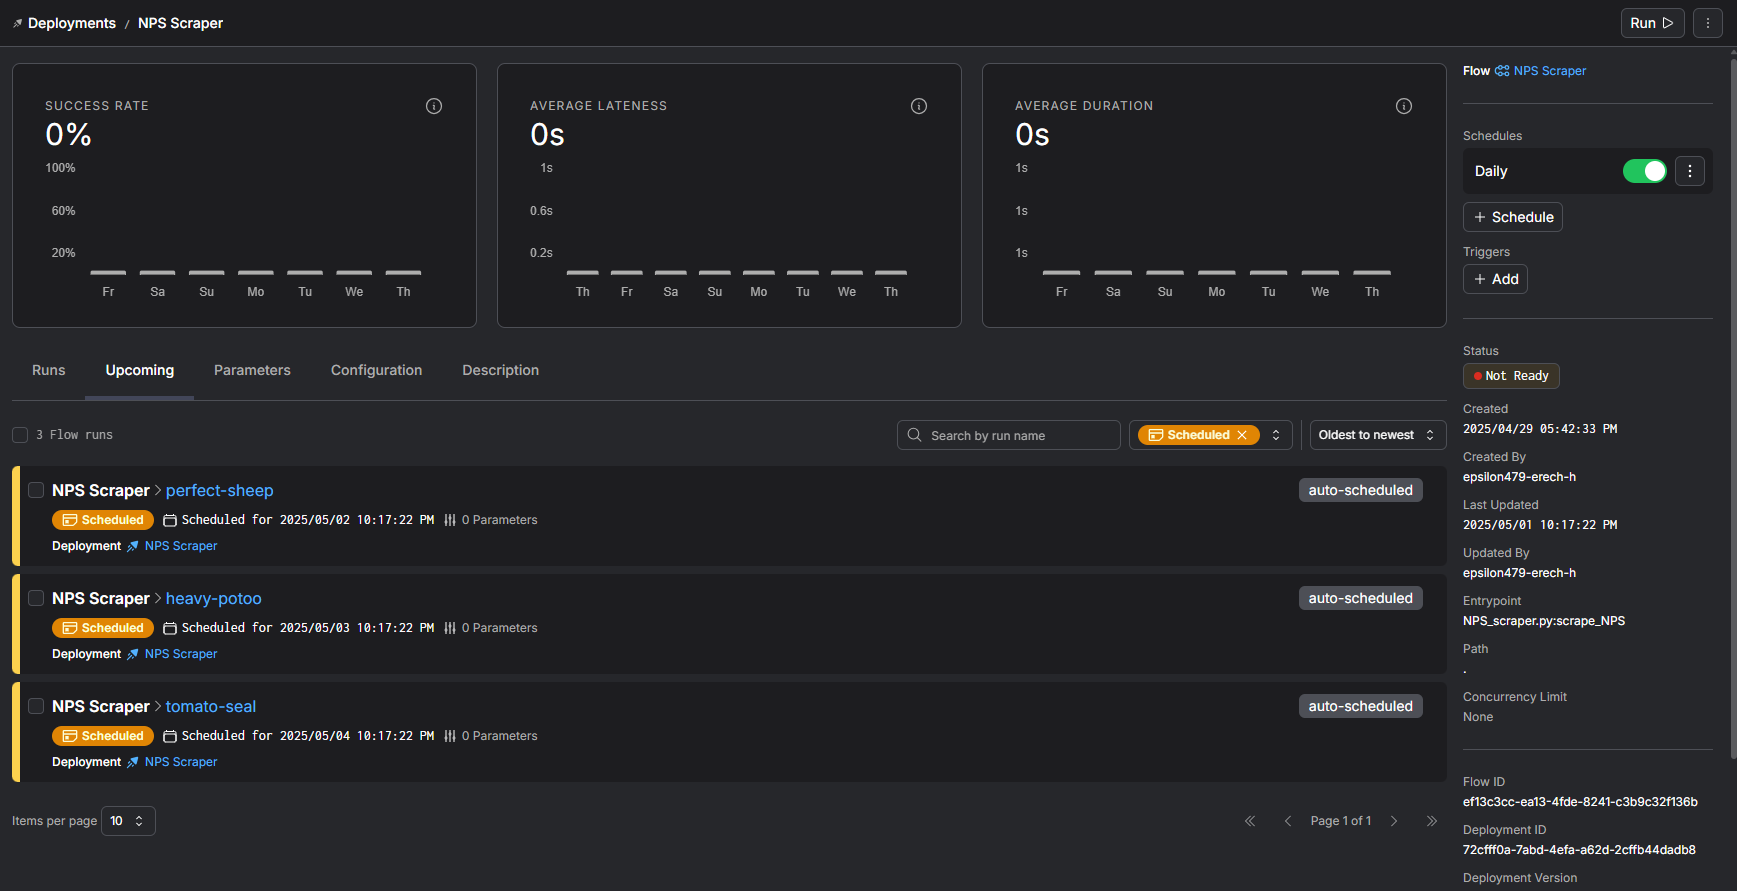
\includegraphics{assets/nps-scraper-deployment.png}

}

\caption{NPS Scraper Deployment in Prefect}

\end{figure}%

\subsubsection{Complete Code}\label{complete-code}

\begin{Shaded}
\begin{Highlighting}[]
\CommentTok{\# Libraries to extract api keys}
\ImportTok{from}\NormalTok{ google.colab }\ImportTok{import}\NormalTok{ userdata}

\CommentTok{\# Get API keys}
\NormalTok{prefect\_api\_key }\OperatorTok{=}\NormalTok{ userdata.get(}\StringTok{"PREFECT\_API\_KEY"}\NormalTok{)}
\NormalTok{nps\_api\_key }\OperatorTok{=}\NormalTok{ userdata.get(}\StringTok{"NPS\_API\_KEY"}\NormalTok{)}
\end{Highlighting}
\end{Shaded}

\begin{Shaded}
\begin{Highlighting}[]
\OperatorTok{\%\%}\NormalTok{capture}
\OperatorTok{!}\NormalTok{pip install prefect}
\end{Highlighting}
\end{Shaded}

\begin{Shaded}
\begin{Highlighting}[]
\OperatorTok{!}\NormalTok{prefect cloud login }\OperatorTok{{-}}\NormalTok{k }\StringTok{"$prefect\_api\_key"}
\end{Highlighting}
\end{Shaded}

\begin{Shaded}
\begin{Highlighting}[]
\CommentTok{\# Libraries used in extraction}
\ImportTok{from}\NormalTok{ pydantic }\ImportTok{import}\NormalTok{ BaseModel, HttpUrl, field\_validator, FilePath}
\ImportTok{from}\NormalTok{ nltk.sentiment.vader }\ImportTok{import}\NormalTok{ SentimentIntensityAnalyzer}
\ImportTok{from}\NormalTok{ prefect.task\_runners }\ImportTok{import}\NormalTok{ ThreadPoolTaskRunner}
\ImportTok{from}\NormalTok{ prefect.futures }\ImportTok{import}\NormalTok{ wait}
\ImportTok{from}\NormalTok{ prefect }\ImportTok{import}\NormalTok{ flow, task}
\ImportTok{from}\NormalTok{ typing }\ImportTok{import}\NormalTok{ List}
\ImportTok{import}\NormalTok{ pandas }\ImportTok{as}\NormalTok{ pd}
\ImportTok{import}\NormalTok{ requests}
\ImportTok{import}\NormalTok{ string}
\ImportTok{import}\NormalTok{ json}
\ImportTok{import}\NormalTok{ nltk}

\CommentTok{\# Download the VADER lexicon for sentiment analysis (quietly)}
\NormalTok{nltk.download(}\StringTok{\textquotesingle{}vader\_lexicon\textquotesingle{}}\NormalTok{, quiet}\OperatorTok{=}\VariableTok{True}\NormalTok{)}

\CommentTok{\# Define Pydantic model for parks}
\KeywordTok{class}\NormalTok{ Park(BaseModel):}
\NormalTok{    fullName: }\BuiltInTok{str} \OperatorTok{|} \VariableTok{None}
\NormalTok{    parkCode: }\BuiltInTok{str} \OperatorTok{|} \VariableTok{None}
\NormalTok{    states: }\BuiltInTok{str} \OperatorTok{|}\NormalTok{ List[}\BuiltInTok{str}\NormalTok{] }\OperatorTok{|} \VariableTok{None}
\NormalTok{    latitude: }\BuiltInTok{float} \OperatorTok{|} \VariableTok{None}
\NormalTok{    longitude: }\BuiltInTok{float} \OperatorTok{|} \VariableTok{None}
\NormalTok{    designation: }\BuiltInTok{str} \OperatorTok{|} \VariableTok{None}
\NormalTok{    url: HttpUrl }\OperatorTok{|} \VariableTok{None}

    \CommentTok{\# Field validator to handle blank values for all fields}
    \AttributeTok{@field\_validator}\NormalTok{(}\StringTok{\textquotesingle{}*\textquotesingle{}}\NormalTok{, mode}\OperatorTok{=}\StringTok{\textquotesingle{}before\textquotesingle{}}\NormalTok{)}
    \AttributeTok{@classmethod}
    \KeywordTok{def}\NormalTok{ clean\_blanks(cls, value: }\BuiltInTok{str} \OperatorTok{|} \BuiltInTok{float}\NormalTok{):}
        \ControlFlowTok{if}\NormalTok{ value }\OperatorTok{==} \StringTok{\textquotesingle{}\textquotesingle{}}\NormalTok{:}
            \ControlFlowTok{return} \VariableTok{None}
        \ControlFlowTok{return}\NormalTok{ value}

\CommentTok{\# Define Pydantic model for activities}
\KeywordTok{class}\NormalTok{ Activity(BaseModel):}
\NormalTok{    parkCode: }\BuiltInTok{str} \OperatorTok{|} \VariableTok{None}
\NormalTok{    activity: List[}\BuiltInTok{str}\NormalTok{] }\OperatorTok{|} \VariableTok{None}

    \CommentTok{\# Field validator to handle blank values for activity fields}
    \AttributeTok{@field\_validator}\NormalTok{(}\StringTok{\textquotesingle{}*\textquotesingle{}}\NormalTok{, mode}\OperatorTok{=}\StringTok{\textquotesingle{}before\textquotesingle{}}\NormalTok{)}
    \AttributeTok{@classmethod}
    \KeywordTok{def}\NormalTok{ clean\_blanks(cls, value: }\BuiltInTok{str} \OperatorTok{|} \BuiltInTok{float}\NormalTok{):}
        \ControlFlowTok{if}\NormalTok{ value }\OperatorTok{==} \StringTok{\textquotesingle{}\textquotesingle{}}\NormalTok{:}
            \ControlFlowTok{return} \VariableTok{None}
        \ControlFlowTok{return}\NormalTok{ value}

\CommentTok{\# Define Pydantic model for alerts}
\KeywordTok{class}\NormalTok{ Alert(BaseModel):}
\NormalTok{    title: }\BuiltInTok{str} \OperatorTok{|} \VariableTok{None}
\NormalTok{    description: }\BuiltInTok{str} \OperatorTok{|} \VariableTok{None}
\NormalTok{    parkCode: }\BuiltInTok{str} \OperatorTok{|} \VariableTok{None}
\NormalTok{    category: }\BuiltInTok{str} \OperatorTok{|} \VariableTok{None}
\NormalTok{    sentiment: }\BuiltInTok{float} \OperatorTok{=} \VariableTok{None}
\NormalTok{    severity: }\BuiltInTok{float} \OperatorTok{=} \VariableTok{None}
\NormalTok{    score: }\BuiltInTok{float} \OperatorTok{=} \VariableTok{None}

    \CommentTok{\# Field validator to handle blank values for alert fields}
    \AttributeTok{@field\_validator}\NormalTok{(}\StringTok{\textquotesingle{}*\textquotesingle{}}\NormalTok{, mode}\OperatorTok{=}\StringTok{\textquotesingle{}before\textquotesingle{}}\NormalTok{)}
    \AttributeTok{@classmethod}
    \KeywordTok{def}\NormalTok{ clean\_blanks(cls, value: }\BuiltInTok{str} \OperatorTok{|} \BuiltInTok{float}\NormalTok{):}
        \ControlFlowTok{if}\NormalTok{ value }\OperatorTok{==} \StringTok{\textquotesingle{}\textquotesingle{}}\NormalTok{:}
            \ControlFlowTok{return} \VariableTok{None}
        \ControlFlowTok{return}\NormalTok{ value}

\CommentTok{\# Function to extract data from the NPS API}
\KeywordTok{def}\NormalTok{ extract\_NPS(endpoint: HttpUrl, verbose: }\BuiltInTok{bool} \OperatorTok{=} \VariableTok{False}\NormalTok{) }\OperatorTok{{-}\textgreater{}}\NormalTok{ List[}\BuiltInTok{dict}\NormalTok{]:}
    \CommentTok{"""}
\CommentTok{    Extract data from the NPS API.}

\CommentTok{    Args:}
\CommentTok{        endpoint (HttpUrl): The URL of the API endpoint to retrieve data from.}
\CommentTok{        verbose (bool): A flag to print detailed information about the request.}

\CommentTok{    Returns:}
\CommentTok{        List[dict]: A list of dictionaries containing the API response data.}
\CommentTok{    """}
    \CommentTok{\# Fetch data from the provided API endpoint}
    \KeywordTok{global}\NormalTok{ nps\_api\_key}
\NormalTok{    headers }\OperatorTok{=}\NormalTok{ \{}\StringTok{"X{-}Api{-}Key"}\NormalTok{: nps\_api\_key\}}
\NormalTok{    response }\OperatorTok{=}\NormalTok{ requests.get(endpoint, headers}\OperatorTok{=}\NormalTok{headers)}
\NormalTok{    data }\OperatorTok{=}\NormalTok{ response.json()}

    \CommentTok{\# Print available data keys if verbose flag is set}
    \ControlFlowTok{if}\NormalTok{ verbose:}
        \BuiltInTok{print}\NormalTok{(}\StringTok{"Keys for request:}\CharTok{\textbackslash{}n}\StringTok{"}\NormalTok{, data.keys())}
        \BuiltInTok{print}\NormalTok{(}\StringTok{"Keys for \textquotesingle{}data\textquotesingle{}:}\CharTok{\textbackslash{}n}\StringTok{"}\NormalTok{, data[}\StringTok{"data"}\NormalTok{][}\DecValTok{0}\NormalTok{].keys())}

    \ControlFlowTok{return}\NormalTok{ data[}\StringTok{"data"}\NormalTok{]}

\CommentTok{\# Function to get park data from the API and return as validated objects}
\AttributeTok{@task}
\KeywordTok{def}\NormalTok{ get\_parks(parks\_endpoint: HttpUrl, verbose: }\BuiltInTok{bool} \OperatorTok{=} \VariableTok{False}\NormalTok{) }\OperatorTok{{-}\textgreater{}}\NormalTok{ List[Park]:}
    \CommentTok{"""}
\CommentTok{    Retrieve park data from the NPS API and return it as validated Park objects.}

\CommentTok{    Args:}
\CommentTok{        parks\_endpoint (HttpUrl): The URL endpoint for fetching park data.}
\CommentTok{        verbose (bool): Flag to enable verbose logging of data retrieval.}

\CommentTok{    Returns:}
\CommentTok{        List[Park]: A list of validated Park Pydantic models.}
\CommentTok{    """}
\NormalTok{    parks\_data }\OperatorTok{=}\NormalTok{ extract\_NPS(parks\_endpoint)}
\NormalTok{    validated\_parks }\OperatorTok{=}\NormalTok{ [Park(}\OperatorTok{**}\NormalTok{park) }\ControlFlowTok{for}\NormalTok{ park }\KeywordTok{in}\NormalTok{ parks\_data]}

    \ControlFlowTok{return}\NormalTok{ validated\_parks}

\CommentTok{\# Function to get alert data from the API and return as validated objects}
\AttributeTok{@task}
\KeywordTok{def}\NormalTok{ get\_alerts(alerts\_endpoint: HttpUrl, verbose: }\BuiltInTok{bool} \OperatorTok{=} \VariableTok{False}\NormalTok{) }\OperatorTok{{-}\textgreater{}}\NormalTok{ List[Alert]:}
    \CommentTok{"""}
\CommentTok{    Retrieve alert data from the NPS API and return it as validated Alert objects.}

\CommentTok{    Args:}
\CommentTok{        alerts\_endpoint (HttpUrl): The URL endpoint for fetching alert data.}
\CommentTok{        verbose (bool): Flag to enable verbose logging of data retrieval.}

\CommentTok{    Returns:}
\CommentTok{        List[Alert]: A list of validated Alert Pydantic models.}
\CommentTok{    """}
\NormalTok{    alerts\_data }\OperatorTok{=}\NormalTok{ extract\_NPS(alerts\_endpoint)}
\NormalTok{    validated\_alerts }\OperatorTok{=}\NormalTok{ [Alert(}\OperatorTok{**}\NormalTok{alert) }\ControlFlowTok{for}\NormalTok{ alert }\KeywordTok{in}\NormalTok{ alerts\_data]}

    \ControlFlowTok{return}\NormalTok{ validated\_alerts}

\CommentTok{\# Function to get activity data from the API, process it, and return as validated objects}
\AttributeTok{@task}
\KeywordTok{def}\NormalTok{ get\_activities(activities\_endpoint: HttpUrl, verbose: }\BuiltInTok{bool} \OperatorTok{=} \VariableTok{False}\NormalTok{) }\OperatorTok{{-}\textgreater{}}\NormalTok{ List[Activity]:}
    \CommentTok{"""}
\CommentTok{    Retrieve activity data from the NPS API, process it into a long format,}
\CommentTok{    and return it as validated Activity objects.}

\CommentTok{    Args:}
\CommentTok{        activities\_endpoint (HttpUrl): The URL endpoint for fetching activity data.}
\CommentTok{        verbose (bool): Flag to enable verbose logging of data retrieval.}

\CommentTok{    Returns:}
\CommentTok{        List[Activity]: A list of validated Activity Pydantic models.}
\CommentTok{    """}
\NormalTok{    activities\_data }\OperatorTok{=}\NormalTok{ extract\_NPS(activities\_endpoint)}
    \CommentTok{\# Unpack activities into a long format DataFrame}
\NormalTok{    df }\OperatorTok{=}\NormalTok{ pd.DataFrame([}
\NormalTok{        \{}\StringTok{\textquotesingle{}activity\textquotesingle{}}\NormalTok{: activity[}\StringTok{\textquotesingle{}name\textquotesingle{}}\NormalTok{], }\StringTok{\textquotesingle{}parkCode\textquotesingle{}}\NormalTok{: park[}\StringTok{\textquotesingle{}parkCode\textquotesingle{}}\NormalTok{]\}}
        \ControlFlowTok{for}\NormalTok{ activity }\KeywordTok{in}\NormalTok{ activities\_data}
        \ControlFlowTok{for}\NormalTok{ park }\KeywordTok{in}\NormalTok{ activity[}\StringTok{\textquotesingle{}parks\textquotesingle{}}\NormalTok{]}
\NormalTok{    ])}
    \CommentTok{\# Group activities by parkCode}
\NormalTok{    df\_grouped }\OperatorTok{=}\NormalTok{ df.groupby(}\StringTok{"parkCode"}\NormalTok{)[}\StringTok{"activity"}\NormalTok{].agg(}\BuiltInTok{list}\NormalTok{).reset\_index()}
\NormalTok{    validated\_activities }\OperatorTok{=}\NormalTok{ [Activity(}\OperatorTok{**}\NormalTok{row) }\ControlFlowTok{for}\NormalTok{ row }\KeywordTok{in}\NormalTok{ df\_grouped.to\_dict(orient}\OperatorTok{=}\StringTok{"records"}\NormalTok{)]}

    \ControlFlowTok{return}\NormalTok{ validated\_activities}

\CommentTok{\# Function to transform alert data by calculating sentiment, severity, and score}
\AttributeTok{@task}
\KeywordTok{def}\NormalTok{ transform\_alerts(alert\_list: List[Alert]) }\OperatorTok{{-}\textgreater{}}\NormalTok{ List[Alert]:}
    \CommentTok{"""}
\CommentTok{    Transform alert data by calculating sentiment, severity, and score for each alert.}

\CommentTok{    Args:}
\CommentTok{        alert\_list (List[Alert]): A list of Alert objects to be processed.}

\CommentTok{    Returns:}
\CommentTok{        List[Alert]: A list of transformed Alert objects with added sentiment, severity, and score attributes.}
\CommentTok{    """}
\NormalTok{    category\_weights }\OperatorTok{=}\NormalTok{ \{}
        \StringTok{\textquotesingle{}Caution\textquotesingle{}}\NormalTok{: }\DecValTok{1}\NormalTok{,}
        \StringTok{\textquotesingle{}Information\textquotesingle{}}\NormalTok{: }\FloatTok{0.5}\NormalTok{,}
        \StringTok{\textquotesingle{}Park Closure\textquotesingle{}}\NormalTok{: }\DecValTok{3}\NormalTok{,}
        \StringTok{\textquotesingle{}Danger\textquotesingle{}}\NormalTok{: }\DecValTok{5}
\NormalTok{    \}}
    \CommentTok{\# Initialize sentiment analysis}
\NormalTok{    analyzer }\OperatorTok{=}\NormalTok{ SentimentIntensityAnalyzer()}
    \CommentTok{\# Calculate sentiment, severity, and score for each alert}
    \ControlFlowTok{for}\NormalTok{ alert\_obj }\KeywordTok{in}\NormalTok{ alert\_list:}
\NormalTok{        sentiment }\OperatorTok{=}\NormalTok{ analyzer.polarity\_scores(alert\_obj.description)[}\StringTok{\textquotesingle{}compound\textquotesingle{}}\NormalTok{]}
\NormalTok{        severity }\OperatorTok{=}\NormalTok{ category\_weights.get(alert\_obj.category, }\DecValTok{0}\NormalTok{)}
\NormalTok{        score }\OperatorTok{=} \BuiltInTok{round}\NormalTok{(severity }\OperatorTok{*}\NormalTok{ (}\DecValTok{1} \OperatorTok{{-}}\NormalTok{ sentiment), }\DecValTok{3}\NormalTok{)}
        \CommentTok{\# Add computed attributes to the alert object}
\NormalTok{        alert\_obj.sentiment }\OperatorTok{=}\NormalTok{ sentiment}
\NormalTok{        alert\_obj.severity }\OperatorTok{=}\NormalTok{ severity}
\NormalTok{        alert\_obj.score }\OperatorTok{=}\NormalTok{ score}

    \ControlFlowTok{return}\NormalTok{ alert\_list}

\CommentTok{\# Function to load data into a file (acting as a database here)}
\AttributeTok{@task}
\KeywordTok{def}\NormalTok{ load\_into\_db(data: List[BaseModel], db\_fpath: FilePath) }\OperatorTok{{-}\textgreater{}} \VariableTok{None}\NormalTok{:}
    \CommentTok{"""}
\CommentTok{    Load a list of data (as Pydantic models) into a file.}

\CommentTok{    Args:}
\CommentTok{        data (List[BaseModel]): A list of Pydantic model objects to be saved.}
\CommentTok{        db\_fpath (FilePath): The file path where the data will be saved.}

\CommentTok{    Returns:}
\CommentTok{        None}
\CommentTok{    """}
    \ControlFlowTok{with} \BuiltInTok{open}\NormalTok{(db\_fpath, }\StringTok{\textquotesingle{}w\textquotesingle{}}\NormalTok{) }\ImportTok{as}\NormalTok{ outfile:}
        \ControlFlowTok{for}\NormalTok{ item }\KeywordTok{in}\NormalTok{ data:}
\NormalTok{            outfile.write(item.model\_dump\_json() }\OperatorTok{+} \StringTok{\textquotesingle{}}\CharTok{\textbackslash{}n}\StringTok{\textquotesingle{}}\NormalTok{)}

\CommentTok{\# Main function to scrape NPS data from multiple endpoints, process it, and save to files}
\AttributeTok{@flow}\NormalTok{(name}\OperatorTok{=}\StringTok{"NPS Scraper"}\NormalTok{) }\CommentTok{\#, task\_runner=ThreadPoolTaskRunner())}
\KeywordTok{def}\NormalTok{ scrape\_NPS(}
\NormalTok{    parks\_endpoint: }\BuiltInTok{str} \OperatorTok{=} \StringTok{"https://developer.nps.gov/api/v1/parks?limit=500"}\NormalTok{,}
\NormalTok{    alerts\_endpoint: }\BuiltInTok{str} \OperatorTok{=} \StringTok{"https://developer.nps.gov/api/v1/alerts?limit=1000"}\NormalTok{,}
\NormalTok{    activities\_endpoint: }\BuiltInTok{str} \OperatorTok{=} \StringTok{"https://developer.nps.gov/api/v1/activities/parks"}\NormalTok{,}
\NormalTok{    parks\_filename: }\BuiltInTok{str} \OperatorTok{=} \StringTok{"extracted\_parks.jsonl"}\NormalTok{,}
\NormalTok{    alerts\_filename: }\BuiltInTok{str} \OperatorTok{=} \StringTok{"extracted\_alerts.jsonl"}\NormalTok{,}
\NormalTok{    activities\_filename: }\BuiltInTok{str} \OperatorTok{=} \StringTok{"extracted\_activities.jsonl"}
\NormalTok{) }\OperatorTok{{-}\textgreater{}} \VariableTok{None}\NormalTok{:}
    \CommentTok{"""}
\CommentTok{    Main flow to scrape NPS data, process it, and save it into files.}

\CommentTok{    Args:}
\CommentTok{        parks\_endpoint (str): The endpoint for fetching park data.}
\CommentTok{        alerts\_endpoint (str): The endpoint for fetching alert data.}
\CommentTok{        activities\_endpoint (str): The endpoint for fetching activity data.}
\CommentTok{        parks\_filename (str): The filename where park data will be saved.}
\CommentTok{        alerts\_filename (str): The filename where alert data will be saved.}
\CommentTok{        activities\_filename (str): The filename where activity data will be saved.}

\CommentTok{    Returns:}
\CommentTok{        None}
\CommentTok{    """}
    \CommentTok{\# Submit tasks concurrently}
\NormalTok{    extracted\_parks }\OperatorTok{=}\NormalTok{ get\_parks(parks\_endpoint)}
\NormalTok{    extracted\_alerts }\OperatorTok{=}\NormalTok{ get\_alerts(alerts\_endpoint)}
\NormalTok{    extracted\_activities }\OperatorTok{=}\NormalTok{ get\_activities(activities\_endpoint)}

    \CommentTok{\# Now transform alerts (depends on extracted\_alerts being ready)}
\NormalTok{    transformed\_alerts }\OperatorTok{=}\NormalTok{ transform\_alerts(extracted\_alerts)}

    \CommentTok{\# Save the extracted and transformed data to separate files}
\NormalTok{    load\_into\_db(extracted\_parks, parks\_filename)}
\NormalTok{    load\_into\_db(transformed\_alerts, alerts\_filename)}
\NormalTok{    load\_into\_db(extracted\_activities, activities\_filename)}

\CommentTok{\# Run the NPS scraping function}
\NormalTok{scrape\_NPS()}
\end{Highlighting}
\end{Shaded}

\begin{Shaded}
\begin{Highlighting}[]
\OperatorTok{\%\%}\NormalTok{writefile NPS\_scraper.py}
\CommentTok{\# Libraries used in extraction}
\ImportTok{from}\NormalTok{ pydantic }\ImportTok{import}\NormalTok{ BaseModel, HttpUrl, field\_validator, FilePath}
\ImportTok{from}\NormalTok{ nltk.sentiment.vader }\ImportTok{import}\NormalTok{ SentimentIntensityAnalyzer}
\ImportTok{from}\NormalTok{ prefect.task\_runners }\ImportTok{import}\NormalTok{ ThreadPoolTaskRunner}
\ImportTok{from}\NormalTok{ prefect.futures }\ImportTok{import}\NormalTok{ wait}
\ImportTok{from}\NormalTok{ prefect }\ImportTok{import}\NormalTok{ flow, task}
\ImportTok{from}\NormalTok{ typing }\ImportTok{import}\NormalTok{ List}
\ImportTok{import}\NormalTok{ pandas }\ImportTok{as}\NormalTok{ pd}
\ImportTok{import}\NormalTok{ requests}
\ImportTok{import}\NormalTok{ string}
\ImportTok{import}\NormalTok{ json}
\ImportTok{import}\NormalTok{ nltk}

\CommentTok{\# Download the VADER lexicon for sentiment analysis (quietly)}
\NormalTok{nltk.download(}\StringTok{\textquotesingle{}vader\_lexicon\textquotesingle{}}\NormalTok{, quiet}\OperatorTok{=}\VariableTok{True}\NormalTok{)}

\CommentTok{\# Define Pydantic model for parks}
\KeywordTok{class}\NormalTok{ Park(BaseModel):}
\NormalTok{    fullName: }\BuiltInTok{str} \OperatorTok{|} \VariableTok{None}
\NormalTok{    parkCode: }\BuiltInTok{str} \OperatorTok{|} \VariableTok{None}
\NormalTok{    states: }\BuiltInTok{str} \OperatorTok{|}\NormalTok{ List[}\BuiltInTok{str}\NormalTok{] }\OperatorTok{|} \VariableTok{None}
\NormalTok{    latitude: }\BuiltInTok{float} \OperatorTok{|} \VariableTok{None}
\NormalTok{    longitude: }\BuiltInTok{float} \OperatorTok{|} \VariableTok{None}
\NormalTok{    designation: }\BuiltInTok{str} \OperatorTok{|} \VariableTok{None}
\NormalTok{    url: HttpUrl }\OperatorTok{|} \VariableTok{None}

    \CommentTok{\# Field validator to handle blank values for all fields}
    \AttributeTok{@field\_validator}\NormalTok{(}\StringTok{\textquotesingle{}*\textquotesingle{}}\NormalTok{, mode}\OperatorTok{=}\StringTok{\textquotesingle{}before\textquotesingle{}}\NormalTok{)}
    \AttributeTok{@classmethod}
    \KeywordTok{def}\NormalTok{ clean\_blanks(cls, value: }\BuiltInTok{str} \OperatorTok{|} \BuiltInTok{float}\NormalTok{):}
        \ControlFlowTok{if}\NormalTok{ value }\OperatorTok{==} \StringTok{\textquotesingle{}\textquotesingle{}}\NormalTok{:}
            \ControlFlowTok{return} \VariableTok{None}
        \ControlFlowTok{return}\NormalTok{ value}

\CommentTok{\# Define Pydantic model for activities}
\KeywordTok{class}\NormalTok{ Activity(BaseModel):}
\NormalTok{    parkCode: }\BuiltInTok{str} \OperatorTok{|} \VariableTok{None}
\NormalTok{    activity: List[}\BuiltInTok{str}\NormalTok{] }\OperatorTok{|} \VariableTok{None}

    \CommentTok{\# Field validator to handle blank values for activity fields}
    \AttributeTok{@field\_validator}\NormalTok{(}\StringTok{\textquotesingle{}*\textquotesingle{}}\NormalTok{, mode}\OperatorTok{=}\StringTok{\textquotesingle{}before\textquotesingle{}}\NormalTok{)}
    \AttributeTok{@classmethod}
    \KeywordTok{def}\NormalTok{ clean\_blanks(cls, value: }\BuiltInTok{str} \OperatorTok{|} \BuiltInTok{float}\NormalTok{):}
        \ControlFlowTok{if}\NormalTok{ value }\OperatorTok{==} \StringTok{\textquotesingle{}\textquotesingle{}}\NormalTok{:}
            \ControlFlowTok{return} \VariableTok{None}
        \ControlFlowTok{return}\NormalTok{ value}

\CommentTok{\# Define Pydantic model for alerts}
\KeywordTok{class}\NormalTok{ Alert(BaseModel):}
\NormalTok{    title: }\BuiltInTok{str} \OperatorTok{|} \VariableTok{None}
\NormalTok{    description: }\BuiltInTok{str} \OperatorTok{|} \VariableTok{None}
\NormalTok{    parkCode: }\BuiltInTok{str} \OperatorTok{|} \VariableTok{None}
\NormalTok{    category: }\BuiltInTok{str} \OperatorTok{|} \VariableTok{None}
\NormalTok{    sentiment: }\BuiltInTok{float} \OperatorTok{=} \VariableTok{None}
\NormalTok{    severity: }\BuiltInTok{float} \OperatorTok{=} \VariableTok{None}
\NormalTok{    score: }\BuiltInTok{float} \OperatorTok{=} \VariableTok{None}

    \CommentTok{\# Field validator to handle blank values for alert fields}
    \AttributeTok{@field\_validator}\NormalTok{(}\StringTok{\textquotesingle{}*\textquotesingle{}}\NormalTok{, mode}\OperatorTok{=}\StringTok{\textquotesingle{}before\textquotesingle{}}\NormalTok{)}
    \AttributeTok{@classmethod}
    \KeywordTok{def}\NormalTok{ clean\_blanks(cls, value: }\BuiltInTok{str} \OperatorTok{|} \BuiltInTok{float}\NormalTok{):}
        \ControlFlowTok{if}\NormalTok{ value }\OperatorTok{==} \StringTok{\textquotesingle{}\textquotesingle{}}\NormalTok{:}
            \ControlFlowTok{return} \VariableTok{None}
        \ControlFlowTok{return}\NormalTok{ value}

\CommentTok{\# Function to extract data from the NPS API}
\KeywordTok{def}\NormalTok{ extract\_NPS(endpoint: HttpUrl, verbose}\OperatorTok{=}\VariableTok{False}\NormalTok{) }\OperatorTok{{-}\textgreater{}}\NormalTok{ List[}\BuiltInTok{dict}\NormalTok{]:}
    \CommentTok{\# Fetch data from the provided API endpoint}
    \KeywordTok{global}\NormalTok{ nps\_api\_key}
\NormalTok{    headers }\OperatorTok{=}\NormalTok{ \{}\StringTok{"X{-}Api{-}Key"}\NormalTok{: nps\_api\_key\}}
\NormalTok{    response }\OperatorTok{=}\NormalTok{ requests.get(endpoint, headers}\OperatorTok{=}\NormalTok{headers)}
\NormalTok{    data }\OperatorTok{=}\NormalTok{ response.json()}

    \CommentTok{\# Print available data keys if verbose flag is set}
    \ControlFlowTok{if}\NormalTok{ verbose:}
        \BuiltInTok{print}\NormalTok{(}\StringTok{"Keys for request:}\CharTok{\textbackslash{}n}\StringTok{"}\NormalTok{, data.keys())}
        \BuiltInTok{print}\NormalTok{(}\StringTok{"Keys for \textquotesingle{}data\textquotesingle{}:}\CharTok{\textbackslash{}n}\StringTok{"}\NormalTok{, data[}\StringTok{"data"}\NormalTok{][}\DecValTok{0}\NormalTok{].keys())}

    \ControlFlowTok{return}\NormalTok{ data[}\StringTok{"data"}\NormalTok{]}

\CommentTok{\# Function to get park data from the API and return as validated objects}
\AttributeTok{@task}
\KeywordTok{def}\NormalTok{ get\_parks(parks\_endpoint: HttpUrl, verbose}\OperatorTok{=}\VariableTok{False}\NormalTok{) }\OperatorTok{{-}\textgreater{}}\NormalTok{ List[Park]:}
\NormalTok{    parks\_data }\OperatorTok{=}\NormalTok{ extract\_NPS(parks\_endpoint)}
\NormalTok{    validated\_parks }\OperatorTok{=}\NormalTok{ [Park(}\OperatorTok{**}\NormalTok{park) }\ControlFlowTok{for}\NormalTok{ park }\KeywordTok{in}\NormalTok{ parks\_data]}

    \ControlFlowTok{return}\NormalTok{ validated\_parks}

\CommentTok{\# Function to get alert data from the API and return as validated objects}
\AttributeTok{@task}
\KeywordTok{def}\NormalTok{ get\_alerts(alerts\_endpoint: HttpUrl, verbose}\OperatorTok{=}\VariableTok{False}\NormalTok{) }\OperatorTok{{-}\textgreater{}}\NormalTok{ List[Alert]:}
\NormalTok{    alerts\_data }\OperatorTok{=}\NormalTok{ extract\_NPS(alerts\_endpoint)}
\NormalTok{    validated\_alerts }\OperatorTok{=}\NormalTok{ [Alert(}\OperatorTok{**}\NormalTok{alert) }\ControlFlowTok{for}\NormalTok{ alert }\KeywordTok{in}\NormalTok{ alerts\_data]}

    \ControlFlowTok{return}\NormalTok{ validated\_alerts}

\CommentTok{\# Function to get activity data from the API, process it, and return as validated objects}
\AttributeTok{@task}
\KeywordTok{def}\NormalTok{ get\_activities(activities\_endpoint: HttpUrl, verbose}\OperatorTok{=}\VariableTok{False}\NormalTok{) }\OperatorTok{{-}\textgreater{}}\NormalTok{ List[Activity]:}
\NormalTok{    activities\_data }\OperatorTok{=}\NormalTok{ extract\_NPS(activities\_endpoint)}
    \CommentTok{\# Unpack activities into a long format DataFrame}
\NormalTok{    df }\OperatorTok{=}\NormalTok{ pd.DataFrame([}
\NormalTok{        \{}\StringTok{\textquotesingle{}activity\textquotesingle{}}\NormalTok{: activity[}\StringTok{\textquotesingle{}name\textquotesingle{}}\NormalTok{], }\StringTok{\textquotesingle{}parkCode\textquotesingle{}}\NormalTok{: park[}\StringTok{\textquotesingle{}parkCode\textquotesingle{}}\NormalTok{]\}}
        \ControlFlowTok{for}\NormalTok{ activity }\KeywordTok{in}\NormalTok{ activities\_data}
        \ControlFlowTok{for}\NormalTok{ park }\KeywordTok{in}\NormalTok{ activity[}\StringTok{\textquotesingle{}parks\textquotesingle{}}\NormalTok{]}
\NormalTok{    ])}
    \CommentTok{\# Group activities by parkCode}
\NormalTok{    df\_grouped }\OperatorTok{=}\NormalTok{ df.groupby(}\StringTok{"parkCode"}\NormalTok{)[}\StringTok{"activity"}\NormalTok{].agg(}\BuiltInTok{list}\NormalTok{).reset\_index()}
\NormalTok{    validated\_activities }\OperatorTok{=}\NormalTok{ [Activity(}\OperatorTok{**}\NormalTok{row) }\ControlFlowTok{for}\NormalTok{ row }\KeywordTok{in}\NormalTok{ df\_grouped.to\_dict(orient}\OperatorTok{=}\StringTok{"records"}\NormalTok{)]}

    \ControlFlowTok{return}\NormalTok{ validated\_activities}

\CommentTok{\# Function to transform alert data by calculating sentiment, severity, and score}
\AttributeTok{@task}
\KeywordTok{def}\NormalTok{ transform\_alerts(alert\_list: List[Alert]) }\OperatorTok{{-}\textgreater{}}\NormalTok{ List[Alert]:}
\NormalTok{    category\_weights }\OperatorTok{=}\NormalTok{ \{}
        \StringTok{\textquotesingle{}Caution\textquotesingle{}}\NormalTok{: }\DecValTok{1}\NormalTok{,}
        \StringTok{\textquotesingle{}Information\textquotesingle{}}\NormalTok{: }\FloatTok{0.5}\NormalTok{,}
        \StringTok{\textquotesingle{}Park Closure\textquotesingle{}}\NormalTok{: }\DecValTok{3}\NormalTok{,}
        \StringTok{\textquotesingle{}Danger\textquotesingle{}}\NormalTok{: }\DecValTok{5}
\NormalTok{    \}}
    \CommentTok{\# Initialize sentiment analysis}
\NormalTok{    analyzer }\OperatorTok{=}\NormalTok{ SentimentIntensityAnalyzer()}
    \CommentTok{\# Calculate sentiment, severity, and score for each alert}
    \ControlFlowTok{for}\NormalTok{ alert\_obj }\KeywordTok{in}\NormalTok{ alert\_list:}
\NormalTok{        sentiment }\OperatorTok{=}\NormalTok{ analyzer.polarity\_scores(alert\_obj.description)[}\StringTok{\textquotesingle{}compound\textquotesingle{}}\NormalTok{]}
\NormalTok{        severity }\OperatorTok{=}\NormalTok{ category\_weights.get(alert\_obj.category, }\DecValTok{0}\NormalTok{)}
\NormalTok{        score }\OperatorTok{=} \BuiltInTok{round}\NormalTok{(severity }\OperatorTok{*}\NormalTok{ (}\DecValTok{1} \OperatorTok{{-}}\NormalTok{ sentiment), }\DecValTok{3}\NormalTok{)}
        \CommentTok{\# Add computed attributes to the alert object}
\NormalTok{        alert\_obj.sentiment }\OperatorTok{=}\NormalTok{ sentiment}
\NormalTok{        alert\_obj.severity }\OperatorTok{=}\NormalTok{ severity}
\NormalTok{        alert\_obj.score }\OperatorTok{=}\NormalTok{ score}

    \ControlFlowTok{return}\NormalTok{ alert\_list}

\CommentTok{\# Function to load data into a file (acting as a database here)}
\AttributeTok{@task}
\KeywordTok{def}\NormalTok{ load\_into\_db(data: List[BaseModel], db\_fpath: FilePath) }\OperatorTok{{-}\textgreater{}} \VariableTok{None}\NormalTok{:}
    \ControlFlowTok{with} \BuiltInTok{open}\NormalTok{(db\_fpath, }\StringTok{\textquotesingle{}w\textquotesingle{}}\NormalTok{) }\ImportTok{as}\NormalTok{ outfile:}
        \ControlFlowTok{for}\NormalTok{ item }\KeywordTok{in}\NormalTok{ data:}
\NormalTok{            outfile.write(item.model\_dump\_json() }\OperatorTok{+} \StringTok{\textquotesingle{}}\CharTok{\textbackslash{}n}\StringTok{\textquotesingle{}}\NormalTok{)}

\CommentTok{\# Main function to scrape NPS data from multiple endpoints, process it, and save to files}
\AttributeTok{@flow}\NormalTok{(name}\OperatorTok{=}\StringTok{"NPS Scraper"}\NormalTok{) }\CommentTok{\#, task\_runner=ThreadPoolTaskRunner())}
\KeywordTok{def}\NormalTok{ scrape\_NPS(}
\NormalTok{    parks\_endpoint: }\BuiltInTok{str} \OperatorTok{=} \StringTok{"https://developer.nps.gov/api/v1/parks?limit=500"}\NormalTok{,}
\NormalTok{    alerts\_endpoint: }\BuiltInTok{str} \OperatorTok{=} \StringTok{"https://developer.nps.gov/api/v1/alerts?limit=1000"}\NormalTok{,}
\NormalTok{    activities\_endpoint: }\BuiltInTok{str} \OperatorTok{=} \StringTok{"https://developer.nps.gov/api/v1/activities/parks"}\NormalTok{,}
\NormalTok{    parks\_filename: }\BuiltInTok{str} \OperatorTok{=} \StringTok{"extracted\_parks.jsonl"}\NormalTok{,}
\NormalTok{    alerts\_filename: }\BuiltInTok{str} \OperatorTok{=} \StringTok{"extracted\_alerts.jsonl"}\NormalTok{,}
\NormalTok{    activities\_filename: }\BuiltInTok{str} \OperatorTok{=} \StringTok{"extracted\_activities.jsonl"}
\NormalTok{) }\OperatorTok{{-}\textgreater{}} \VariableTok{None}\NormalTok{:}
     \CommentTok{\# Submit tasks concurrently}
\NormalTok{    extracted\_parks }\OperatorTok{=}\NormalTok{ get\_parks(parks\_endpoint)}
\NormalTok{    extracted\_alerts }\OperatorTok{=}\NormalTok{ get\_alerts(alerts\_endpoint)}
\NormalTok{    extracted\_activities }\OperatorTok{=}\NormalTok{ get\_activities(activities\_endpoint)}

    \CommentTok{\# Now transform alerts (depends on extracted\_alerts being ready)}
\NormalTok{    transformed\_alerts }\OperatorTok{=}\NormalTok{ transform\_alerts(extracted\_alerts)}

    \CommentTok{\# Save the extracted and transformed data to separate files}
\NormalTok{    load\_into\_db(extracted\_parks, parks\_filename)}
\NormalTok{    load\_into\_db(transformed\_alerts, alerts\_filename)}
\NormalTok{    load\_into\_db(extracted\_activities, activities\_filename)}


\ControlFlowTok{if} \VariableTok{\_\_name\_\_} \OperatorTok{==} \StringTok{"\_\_main\_\_"}\NormalTok{:}
\NormalTok{  scrape\_NPS.serve(}
\NormalTok{      name}\OperatorTok{=}\StringTok{"NPS Scraper"}\NormalTok{,}
\NormalTok{      interval }\OperatorTok{=}\NormalTok{ (}\DecValTok{60}\OperatorTok{*}\DecValTok{60}\OperatorTok{*}\DecValTok{24}\NormalTok{) }\CommentTok{\# once weekly}
\NormalTok{)}
\end{Highlighting}
\end{Shaded}

\begin{Shaded}
\begin{Highlighting}[]
\OperatorTok{!}\NormalTok{python NPS\_scraper.py}
\end{Highlighting}
\end{Shaded}

\begin{Shaded}
\begin{Highlighting}[]
\CommentTok{\# Import necessary libraries}
\ImportTok{from}\NormalTok{ prefect.artifacts }\ImportTok{import}\NormalTok{ create\_markdown\_artifact, create\_link\_artifact}
\ImportTok{from}\NormalTok{ urllib.parse }\ImportTok{import}\NormalTok{ urljoin}
\ImportTok{from}\NormalTok{ bs4 }\ImportTok{import}\NormalTok{ BeautifulSoup}
\ImportTok{from}\NormalTok{ prefect }\ImportTok{import}\NormalTok{ flow, task}
\ImportTok{from}\NormalTok{ pydantic }\ImportTok{import}\NormalTok{ HttpUrl}
\ImportTok{from}\NormalTok{ typing }\ImportTok{import}\NormalTok{ List}
\ImportTok{import}\NormalTok{ pandas }\ImportTok{as}\NormalTok{ pd}
\ImportTok{import}\NormalTok{ datetime}
\ImportTok{import}\NormalTok{ requests}
\ImportTok{import}\NormalTok{ re}
\CommentTok{\# for map}
\ImportTok{from}\NormalTok{ branca.colormap }\ImportTok{import}\NormalTok{ LinearColormap}
\ImportTok{from}\NormalTok{ folium.plugins }\ImportTok{import}\NormalTok{ MarkerCluster}
\ImportTok{from}\NormalTok{ ftplib }\ImportTok{import}\NormalTok{ FTP\_TLS}
\ImportTok{import}\NormalTok{ folium}

\CommentTok{\# Function to load and merge the datasets (parks, alerts, and activities)}
\AttributeTok{@task}
\KeywordTok{def}\NormalTok{ load\_and\_merge(}
\NormalTok{        parks\_file: }\BuiltInTok{str}\NormalTok{,}
\NormalTok{        alerts\_file: }\BuiltInTok{str}\NormalTok{,}
\NormalTok{        activities\_file: }\BuiltInTok{str}
\NormalTok{    ) }\OperatorTok{{-}\textgreater{}}\NormalTok{ pd.DataFrame:}
    \CommentTok{"""}
\CommentTok{    Loads and merges park, alert, and activity data from the specified JSONL files.}

\CommentTok{    Args:}
\CommentTok{        parks\_file (str): Path to the parks data file (in JSONL format).}
\CommentTok{        alerts\_file (str): Path to the alerts data file (in JSONL format).}
\CommentTok{        activities\_file (str): Path to the activities data file (in JSONL format).}

\CommentTok{    Returns:}
\CommentTok{        pd.DataFrame: A merged DataFrame containing parks, alerts, and activities data.}
\CommentTok{    """}
    \CommentTok{\# Read in the JSONL files containing parks, alerts, and activities data}
\NormalTok{    parks\_df }\OperatorTok{=}\NormalTok{ pd.read\_json(parks\_file, lines}\OperatorTok{=}\VariableTok{True}\NormalTok{)}
\NormalTok{    alerts\_df }\OperatorTok{=}\NormalTok{ pd.read\_json(alerts\_file, lines}\OperatorTok{=}\VariableTok{True}\NormalTok{)}
\NormalTok{    activities\_df }\OperatorTok{=}\NormalTok{ pd.read\_json(activities\_file, lines}\OperatorTok{=}\VariableTok{True}\NormalTok{)}

    \CommentTok{\# Categorize the designations of parks}
\NormalTok{    parks\_df }\OperatorTok{=}\NormalTok{ categorize\_designations(parks\_df)}

    \CommentTok{\# Merge parks data with activities data based on park code}
\NormalTok{    merged\_df }\OperatorTok{=}\NormalTok{ pd.merge(parks\_df, activities\_df, on}\OperatorTok{=}\StringTok{"parkCode"}\NormalTok{, how}\OperatorTok{=}\StringTok{"left"}\NormalTok{)}

    \CommentTok{\# Merge the result with the alerts data}
\NormalTok{    final\_df }\OperatorTok{=}\NormalTok{ pd.merge(merged\_df, alerts\_df, on}\OperatorTok{=}\StringTok{"parkCode"}\NormalTok{, how}\OperatorTok{=}\StringTok{"right"}\NormalTok{)}

    \CommentTok{\# Return the final merged DataFrame}
    \ControlFlowTok{return}\NormalTok{ final\_df}

\CommentTok{\# Function to categorize parks based on their designations}
\KeywordTok{def}\NormalTok{ categorize\_designations(parks\_df: pd.DataFrame) }\OperatorTok{{-}\textgreater{}}\NormalTok{ pd.DataFrame:}
    \CommentTok{"""}
\CommentTok{    Categorizes parks based on their designations into predefined categories.}

\CommentTok{    Args:}
\CommentTok{        parks\_df (pd.DataFrame): A DataFrame containing park data.}

\CommentTok{    Returns:}
\CommentTok{        pd.DataFrame: The input DataFrame with an added \textquotesingle{}designation\textquotesingle{} column for park categories.}
\CommentTok{    """}
    \CommentTok{\# Define the categories and corresponding designations}
\NormalTok{    designation\_categories }\OperatorTok{=}\NormalTok{ \{}
        \StringTok{"National Park or Preserve"}\NormalTok{: [}
            \StringTok{\textquotesingle{}National Park\textquotesingle{}}\NormalTok{, }\StringTok{\textquotesingle{}National Parks\textquotesingle{}}\NormalTok{, }\StringTok{\textquotesingle{}National Park \& Preserve\textquotesingle{}}\NormalTok{,}
            \StringTok{\textquotesingle{}National Preserve\textquotesingle{}}\NormalTok{, }\StringTok{\textquotesingle{}National and State Parks\textquotesingle{}}
\NormalTok{        ],}
        \StringTok{"Monument or Memorial"}\NormalTok{: [}
            \StringTok{\textquotesingle{}National Monument\textquotesingle{}}\NormalTok{, }\StringTok{\textquotesingle{}National Monument and Historic Shrine\textquotesingle{}}\NormalTok{,}
            \StringTok{\textquotesingle{}National Memorial\textquotesingle{}}\NormalTok{, }\StringTok{\textquotesingle{}National Monument \& Preserve\textquotesingle{}}\NormalTok{,}
            \StringTok{\textquotesingle{}Part of Statue of Liberty National Monument\textquotesingle{}}
\NormalTok{        ],}
        \StringTok{"Historic or Cultural Site"}\NormalTok{: [}
            \StringTok{\textquotesingle{}National Historic Site\textquotesingle{}}\NormalTok{, }\StringTok{\textquotesingle{}National Historical Park\textquotesingle{}}\NormalTok{,}
            \StringTok{\textquotesingle{}National Historical Park and Ecological Preserve\textquotesingle{}}\NormalTok{,}
            \StringTok{\textquotesingle{}International Historic Site\textquotesingle{}}\NormalTok{, }\StringTok{\textquotesingle{}National Historical Park and Preserve\textquotesingle{}}\NormalTok{,}
            \StringTok{\textquotesingle{}Part of Colonial National Historical Park\textquotesingle{}}
\NormalTok{        ],}
        \StringTok{"Water{-}Based or Natural Area"}\NormalTok{: [}
            \StringTok{\textquotesingle{}National Seashore\textquotesingle{}}\NormalTok{, }\StringTok{\textquotesingle{}National Lakeshore\textquotesingle{}}\NormalTok{, }\StringTok{\textquotesingle{}National River\textquotesingle{}}\NormalTok{,}
            \StringTok{\textquotesingle{}National Scenic River\textquotesingle{}}\NormalTok{, }\StringTok{\textquotesingle{}National Scenic Riverway\textquotesingle{}}\NormalTok{,}
            \StringTok{\textquotesingle{}National Scenic Riverways\textquotesingle{}}\NormalTok{, }\StringTok{\textquotesingle{}National Recreational River\textquotesingle{}}\NormalTok{,}
            \StringTok{\textquotesingle{}Scenic \& Recreational River\textquotesingle{}}\NormalTok{, }\StringTok{\textquotesingle{}National River \& Recreation Area\textquotesingle{}}\NormalTok{,}
            \StringTok{\textquotesingle{}National Recreation Area\textquotesingle{}}\NormalTok{, }\StringTok{\textquotesingle{}International Park\textquotesingle{}}\NormalTok{, }\StringTok{\textquotesingle{}Park\textquotesingle{}}
\NormalTok{        ],}
        \StringTok{"Trail, Parkway, or Battlefield"}\NormalTok{: [}
            \StringTok{\textquotesingle{}National Historic Trail\textquotesingle{}}\NormalTok{, }\StringTok{\textquotesingle{}National Scenic Trail\textquotesingle{}}\NormalTok{, }\StringTok{\textquotesingle{}Parkway\textquotesingle{}}\NormalTok{,}
            \StringTok{\textquotesingle{}Memorial Parkway\textquotesingle{}}\NormalTok{, }\StringTok{\textquotesingle{}National Battlefield\textquotesingle{}}\NormalTok{,}
            \StringTok{\textquotesingle{}National Battlefield Park\textquotesingle{}}\NormalTok{, }\StringTok{\textquotesingle{}National Military Park\textquotesingle{}}
\NormalTok{        ]}
\NormalTok{    \}}

    \CommentTok{\# Create a mapping from designations to categories}
\NormalTok{    designation\_map }\OperatorTok{=}\NormalTok{ \{}
\NormalTok{        designation: category}
        \ControlFlowTok{for}\NormalTok{ category, designations }\KeywordTok{in}\NormalTok{ designation\_categories.items()}
        \ControlFlowTok{for}\NormalTok{ designation }\KeywordTok{in}\NormalTok{ designations}
\NormalTok{    \}}

    \CommentTok{\# Apply the mapping to categorize the parks}
\NormalTok{    parks\_df[}\StringTok{\textquotesingle{}designation\textquotesingle{}}\NormalTok{] }\OperatorTok{=}\NormalTok{ parks\_df[}\StringTok{\textquotesingle{}designation\textquotesingle{}}\NormalTok{].}\BuiltInTok{map}\NormalTok{(designation\_map).fillna(}\StringTok{\textquotesingle{}Other\textquotesingle{}}\NormalTok{)}

    \CommentTok{\# Return the updated parks DataFrame}
    \ControlFlowTok{return}\NormalTok{ parks\_df}

\CommentTok{\# Function to get the most common alert types from the alerts DataFrame}
\KeywordTok{def}\NormalTok{ get\_top\_alert\_types(df: pd.DataFrame) }\OperatorTok{{-}\textgreater{}} \BuiltInTok{str}\NormalTok{:}
    \CommentTok{"""}
\CommentTok{    Extracts the most common alert types from the provided DataFrame.}

\CommentTok{    Args:}
\CommentTok{        df (pd.DataFrame): A DataFrame containing alerts data.}

\CommentTok{    Returns:}
\CommentTok{        str: A markdown string representing the most common alert types and their counts.}
\CommentTok{    """}
\NormalTok{    top\_alert\_df }\OperatorTok{=}\NormalTok{ df[}\StringTok{\textquotesingle{}category\textquotesingle{}}\NormalTok{].value\_counts().reset\_index()}
\NormalTok{    top\_alert\_df.columns }\OperatorTok{=}\NormalTok{ [}\StringTok{\textquotesingle{}Category\textquotesingle{}}\NormalTok{, }\StringTok{\textquotesingle{}Count\textquotesingle{}}\NormalTok{]}
\NormalTok{    top\_alert\_md }\OperatorTok{=}\NormalTok{ top\_alert\_df.to\_markdown(index}\OperatorTok{=}\VariableTok{False}\NormalTok{)}
    \ControlFlowTok{return}\NormalTok{ top\_alert\_md}

\CommentTok{\# Function to get the top sites based on a specific metric (e.g., number of alerts or alert score)}
\KeywordTok{def}\NormalTok{ get\_top\_sites(}
\NormalTok{        df: pd.DataFrame,}
\NormalTok{        by: }\BuiltInTok{str}\NormalTok{,}
\NormalTok{        site\_type: }\BuiltInTok{str}\NormalTok{,}
\NormalTok{        top\_n: }\BuiltInTok{int}\NormalTok{,}
\NormalTok{        ascending: }\BuiltInTok{bool} \OperatorTok{=} \VariableTok{False}
\NormalTok{    ) }\OperatorTok{{-}\textgreater{}} \BuiltInTok{str}\NormalTok{:}
    \CommentTok{"""}
\CommentTok{    Retrieves the top N sites based on a specified metric (e.g., number of alerts or alert score).}

\CommentTok{    Args:}
\CommentTok{        df (pd.DataFrame): A DataFrame containing site data.}
\CommentTok{        by (str): The metric column to sort by (e.g., \textquotesingle{}num\_alerts\textquotesingle{}, \textquotesingle{}score\textquotesingle{}).}
\CommentTok{        site\_type (str): The type of sites to filter by (e.g., \textquotesingle{}National Park\textquotesingle{}).}
\CommentTok{        top\_n (int): The number of top sites to retrieve.}
\CommentTok{        ascending (bool, optional): Whether to sort in ascending order (default is False).}

\CommentTok{    Returns:}
\CommentTok{        str: A markdown table of the top sites with the specified metric.}
\CommentTok{    """}
    \CommentTok{\# Aggregate the data for the specified site type}
\NormalTok{    agg\_df }\OperatorTok{=}\NormalTok{ aggregate\_data(df, site\_type)}

    \CommentTok{\# Keep only relevant columns}
\NormalTok{    keep\_cols }\OperatorTok{=}\NormalTok{ [}\StringTok{\textquotesingle{}fullName\textquotesingle{}}\NormalTok{, }\StringTok{\textquotesingle{}states\textquotesingle{}}\NormalTok{, }\StringTok{\textquotesingle{}url\textquotesingle{}}\NormalTok{, }\StringTok{\textquotesingle{}sentiment\textquotesingle{}}\NormalTok{, }\StringTok{\textquotesingle{}severity\textquotesingle{}}\NormalTok{, by]}
\NormalTok{    agg\_df }\OperatorTok{=}\NormalTok{ agg\_df[keep\_cols]}

    \CommentTok{\# Sort the DataFrame based on the specified metric (ascending or descending)}
\NormalTok{    sorted\_df }\OperatorTok{=}\NormalTok{ agg\_df.sort\_values(by}\OperatorTok{=}\NormalTok{by, ascending}\OperatorTok{=}\NormalTok{ascending).head(top\_n)}

    \CommentTok{\# Convert the sorted DataFrame to a markdown table}
\NormalTok{    md\_table }\OperatorTok{=}\NormalTok{ create\_md\_table(sorted\_df, keep\_cols)}

    \ControlFlowTok{return}\NormalTok{ md\_table}

\CommentTok{\# Function to aggregate alert data for a specific site type}
\KeywordTok{def}\NormalTok{ aggregate\_data(df: pd.DataFrame, site\_type: }\BuiltInTok{str}\NormalTok{) }\OperatorTok{{-}\textgreater{}}\NormalTok{ pd.DataFrame:}
    \CommentTok{"""}
\CommentTok{    Aggregates alert data for a specific site type and calculates average sentiment, severity,}
\CommentTok{    total score, and the number of alerts.}

\CommentTok{    Args:}
\CommentTok{        df (pd.DataFrame): A DataFrame containing alerts data.}
\CommentTok{        site\_type (str): The site type to filter by (e.g., \textquotesingle{}National Park\textquotesingle{}).}

\CommentTok{    Returns:}
\CommentTok{        pd.DataFrame: A DataFrame containing aggregated alert data for the specified site type.}
\CommentTok{    """}
    \CommentTok{\# Filter the DataFrame by the specified site type}
\NormalTok{    df }\OperatorTok{=}\NormalTok{ df[df[}\StringTok{\textquotesingle{}designation\textquotesingle{}}\NormalTok{] }\OperatorTok{==}\NormalTok{ site\_type]}

    \CommentTok{\# Aggregate the data (average sentiment, severity, total score, and number of alerts)}
\NormalTok{    agg\_df }\OperatorTok{=}\NormalTok{ df.groupby([}\StringTok{\textquotesingle{}fullName\textquotesingle{}}\NormalTok{, }\StringTok{\textquotesingle{}states\textquotesingle{}}\NormalTok{, }\StringTok{\textquotesingle{}url\textquotesingle{}}\NormalTok{]).agg(\{}
        \StringTok{\textquotesingle{}sentiment\textquotesingle{}}\NormalTok{: }\StringTok{\textquotesingle{}mean\textquotesingle{}}\NormalTok{,}
        \StringTok{\textquotesingle{}severity\textquotesingle{}}\NormalTok{: }\StringTok{\textquotesingle{}mean\textquotesingle{}}\NormalTok{,}
        \StringTok{\textquotesingle{}score\textquotesingle{}}\NormalTok{: }\StringTok{\textquotesingle{}sum\textquotesingle{}}\NormalTok{,}
        \StringTok{\textquotesingle{}fullName\textquotesingle{}}\NormalTok{: }\StringTok{\textquotesingle{}size\textquotesingle{}}
\NormalTok{    \}).rename(columns}\OperatorTok{=}\NormalTok{\{}\StringTok{\textquotesingle{}fullName\textquotesingle{}}\NormalTok{: }\StringTok{\textquotesingle{}num\_alerts\textquotesingle{}}\NormalTok{\}).reset\_index()}

    \CommentTok{\# Normalize the score for readability}
\NormalTok{    agg\_df[}\StringTok{"score"}\NormalTok{] }\OperatorTok{=} \BuiltInTok{round}\NormalTok{((agg\_df[}\StringTok{"score"}\NormalTok{] }\OperatorTok{{-}} \BuiltInTok{min}\NormalTok{(agg\_df[}\StringTok{"score"}\NormalTok{])) }\OperatorTok{/}\NormalTok{ (}\BuiltInTok{max}\NormalTok{(agg\_df[}\StringTok{"score"}\NormalTok{]) }\OperatorTok{{-}} \BuiltInTok{min}\NormalTok{(agg\_df[}\StringTok{"score"}\NormalTok{])), }\DecValTok{4}\NormalTok{) }\OperatorTok{*} \DecValTok{100}

    \ControlFlowTok{return}\NormalTok{ agg\_df}

\CommentTok{\# Function to create a markdown table from the sorted DataFrame}
\KeywordTok{def}\NormalTok{ create\_md\_table(sorted\_df: pd.DataFrame, keep\_cols: List[}\BuiltInTok{str}\NormalTok{]) }\OperatorTok{{-}\textgreater{}} \BuiltInTok{str}\NormalTok{:}
    \CommentTok{"""}
\CommentTok{    Converts the sorted DataFrame into a markdown table.}

\CommentTok{    Args:}
\CommentTok{        sorted\_df (pd.DataFrame): The sorted DataFrame containing site data.}
\CommentTok{        keep\_cols (List[str]): The list of columns to include in the markdown table.}

\CommentTok{    Returns:}
\CommentTok{        str: A markdown{-}formatted table as a string.}
\CommentTok{    """}
    \CommentTok{\# Map the column names to user{-}friendly names}
\NormalTok{    rename\_map }\OperatorTok{=}\NormalTok{ \{}
        \StringTok{\textquotesingle{}fullName\textquotesingle{}}\NormalTok{: }\StringTok{\textquotesingle{}Site Name\textquotesingle{}}\NormalTok{,}
        \StringTok{\textquotesingle{}states\textquotesingle{}}\NormalTok{: }\StringTok{\textquotesingle{}State(s)\textquotesingle{}}\NormalTok{,}
        \StringTok{\textquotesingle{}url\textquotesingle{}}\NormalTok{: }\StringTok{\textquotesingle{}Site Website\textquotesingle{}}\NormalTok{,}
        \StringTok{\textquotesingle{}sentiment\textquotesingle{}}\NormalTok{: }\StringTok{\textquotesingle{}Avg. Sentiment\textquotesingle{}}\NormalTok{,}
        \StringTok{\textquotesingle{}severity\textquotesingle{}}\NormalTok{: }\StringTok{\textquotesingle{}Avg. Severity\textquotesingle{}}\NormalTok{,}
        \StringTok{\textquotesingle{}score\textquotesingle{}}\NormalTok{: }\StringTok{\textquotesingle{}Alert Score\textquotesingle{}}\NormalTok{,}
        \StringTok{\textquotesingle{}num\_alerts\textquotesingle{}}\NormalTok{: }\StringTok{\textquotesingle{}Number of Alerts\textquotesingle{}}
\NormalTok{    \}}
\NormalTok{    rename\_map }\OperatorTok{=}\NormalTok{ \{k:v }\ControlFlowTok{for}\NormalTok{ k,v }\KeywordTok{in}\NormalTok{ rename\_map.items() }\ControlFlowTok{if}\NormalTok{ k }\KeywordTok{in}\NormalTok{ keep\_cols\}}

    \CommentTok{\# Rename columns}
\NormalTok{    sorted\_df }\OperatorTok{=}\NormalTok{ sorted\_df.rename(columns}\OperatorTok{=}\NormalTok{rename\_map).reset\_index(drop}\OperatorTok{=}\VariableTok{True}\NormalTok{)}

    \CommentTok{\# Set the index to start from 1 for display purposes}
\NormalTok{    sorted\_df.index }\OperatorTok{=}\NormalTok{ sorted\_df.index }\OperatorTok{+} \DecValTok{1}

    \CommentTok{\# Convert the DataFrame to a markdown table}
\NormalTok{    md\_table }\OperatorTok{=}\NormalTok{ sorted\_df.to\_markdown()}

    \ControlFlowTok{return}\NormalTok{ md\_table}

\CommentTok{\# Function to get top images from a park website}
\KeywordTok{def}\NormalTok{ get\_top\_images(park\_url: HttpUrl) }\OperatorTok{{-}\textgreater{}} \BuiltInTok{str}\NormalTok{:}
    \CommentTok{"""}
\CommentTok{    Retrieves the top image from a park\textquotesingle{}s website by scraping the HTML content.}

\CommentTok{    Args:}
\CommentTok{        park\_url (HttpUrl): The URL of the park\textquotesingle{}s website.}

\CommentTok{    Returns:}
\CommentTok{        str: HTML image tag containing the top image for the park.}
\CommentTok{    """}
    \CommentTok{\# Fetch the webpage content}
\NormalTok{    page\_url }\OperatorTok{=}\NormalTok{ park\_url}
\NormalTok{    response }\OperatorTok{=}\NormalTok{ requests.get(page\_url)}
\NormalTok{    soup }\OperatorTok{=}\NormalTok{ BeautifulSoup(response.text, }\StringTok{\textquotesingle{}html.parser\textquotesingle{}}\NormalTok{)}

    \CommentTok{\# Find the div containing the background image}
\NormalTok{    div }\OperatorTok{=}\NormalTok{ soup.find(}\StringTok{\textquotesingle{}div\textquotesingle{}}\NormalTok{, class\_}\OperatorTok{=}\StringTok{\textquotesingle{}picturefill{-}background\textquotesingle{}}\NormalTok{)}
\NormalTok{    style }\OperatorTok{=}\NormalTok{ div.get(}\StringTok{\textquotesingle{}style\textquotesingle{}}\NormalTok{)}

    \CommentTok{\# Extract the image URL from the style attribute}
\NormalTok{    match\_url }\OperatorTok{=}\NormalTok{ re.search(}\VerbatimStringTok{r"url\textbackslash{}(\textquotesingle{}(.*?)\textquotesingle{}\textbackslash{})"}\NormalTok{, style)}
\NormalTok{    relative\_img\_url }\OperatorTok{=}\NormalTok{ match\_url.group(}\DecValTok{1}\NormalTok{)}

    \CommentTok{\# Build the full image URL and return HTML for embedding the image}
\NormalTok{    full\_img\_url }\OperatorTok{=}\NormalTok{ urljoin(}\StringTok{\textquotesingle{}https://www.nps.gov\textquotesingle{}}\NormalTok{, relative\_img\_url)}
\NormalTok{    img\_html }\OperatorTok{=} \SpecialStringTok{f"""\textless{}img src="}\SpecialCharTok{\{}\NormalTok{full\_img\_url}\SpecialCharTok{\}}\SpecialStringTok{" alt="Image at Site" width="500"\textgreater{}}\CharTok{\textbackslash{}n\textbackslash{}n}\SpecialStringTok{"""}

    \ControlFlowTok{return}\NormalTok{ img\_html}

\CommentTok{\# Function to get popular activities at top sites}
\KeywordTok{def}\NormalTok{ get\_top\_activities(df: pd.DataFrame, site\_type: }\BuiltInTok{str}\NormalTok{, top\_n: }\BuiltInTok{int} \OperatorTok{=} \DecValTok{5}\NormalTok{) }\OperatorTok{{-}\textgreater{}} \BuiltInTok{str}\NormalTok{:}
    \CommentTok{"""}
\CommentTok{    Retrieves the most popular activities at the top sites based on alert scores.}

\CommentTok{    Args:}
\CommentTok{        df (pd.DataFrame): A DataFrame containing park and activity data.}
\CommentTok{        site\_type (str): The site type to filter by (e.g., \textquotesingle{}National Park\textquotesingle{}).}
\CommentTok{        top\_n (int, optional): The number of top activities to return (default is 5).}

\CommentTok{    Returns:}
\CommentTok{        str: A markdown string containing popular activities at top sites.}
\CommentTok{    """}
    \CommentTok{\# Aggregate data to get the top parks based on the score}
\NormalTok{    agg\_df }\OperatorTok{=}\NormalTok{ aggregate\_data(df, site\_type)}
\NormalTok{    top\_parks }\OperatorTok{=}\NormalTok{ agg\_df.sort\_values(}\StringTok{"score"}\NormalTok{).head(top\_n)}

    \CommentTok{\# Filter the original DataFrame to get data for top parks}
\NormalTok{    top\_park\_names }\OperatorTok{=}\NormalTok{ top\_parks[}\StringTok{\textquotesingle{}fullName\textquotesingle{}}\NormalTok{].tolist()}
\NormalTok{    top\_df }\OperatorTok{=}\NormalTok{ df[df[}\StringTok{\textquotesingle{}fullName\textquotesingle{}}\NormalTok{].isin(top\_park\_names)][[}\StringTok{\textquotesingle{}fullName\textquotesingle{}}\NormalTok{, }\StringTok{\textquotesingle{}url\textquotesingle{}}\NormalTok{, }\StringTok{\textquotesingle{}activity\textquotesingle{}}\NormalTok{]]}

    \CommentTok{\# Prepare markdown content for activities}
\NormalTok{    activity\_md }\OperatorTok{=} \StringTok{""}
    \ControlFlowTok{for}\NormalTok{ idx, row }\KeywordTok{in}\NormalTok{ top\_df.iterrows():}
\NormalTok{        activity\_md }\OperatorTok{+=}\NormalTok{ get\_top\_images(row[}\StringTok{\textquotesingle{}url\textquotesingle{}}\NormalTok{])}
\NormalTok{        activity\_md }\OperatorTok{+=} \SpecialStringTok{f"\#\#\# }\SpecialCharTok{\{}\NormalTok{row[}\StringTok{\textquotesingle{}fullName\textquotesingle{}}\NormalTok{]}\SpecialCharTok{\}}\CharTok{\textbackslash{}n}\SpecialStringTok{"}
        \ControlFlowTok{for}\NormalTok{ acts }\KeywordTok{in}\NormalTok{ row[}\StringTok{\textquotesingle{}activity\textquotesingle{}}\NormalTok{]:}
\NormalTok{            activity\_md }\OperatorTok{+=} \SpecialStringTok{f"{-} }\SpecialCharTok{\{}\NormalTok{acts}\SpecialCharTok{\}}\CharTok{\textbackslash{}n}\SpecialStringTok{"}

\NormalTok{        activity\_md }\OperatorTok{+=} \SpecialStringTok{f"}\CharTok{\textbackslash{}n}\SpecialStringTok{\textless{}br\textgreater{}}\CharTok{\textbackslash{}n}\SpecialStringTok{\textless{}br\textgreater{}}\CharTok{\textbackslash{}n}\SpecialStringTok{"}

    \ControlFlowTok{return}\NormalTok{ activity\_md}

\CommentTok{\# task function to generate the full report}
\AttributeTok{@task}
\KeywordTok{def}\NormalTok{ load\_into\_report(}
\NormalTok{        df: pd.DataFrame,}
\NormalTok{        site\_type: }\BuiltInTok{str}\NormalTok{,}
\NormalTok{        top\_n: }\BuiltInTok{int} \OperatorTok{=} \DecValTok{10}
\NormalTok{    ) }\OperatorTok{{-}\textgreater{}} \BuiltInTok{str}\NormalTok{:}
    \CommentTok{"""}
\CommentTok{    Generates a markdown report summarizing the top alert types, sites with the most alerts,}
\CommentTok{    sites with the highest alert scores, and popular activities at the top sites.}

\CommentTok{    Args:}
\CommentTok{        df (pd.DataFrame): The merged DataFrame containing parks, alerts, and activities data.}
\CommentTok{        site\_type (str): The type of sites to report on (e.g., \textquotesingle{}National Park\textquotesingle{}).}
\CommentTok{        top\_n (int, optional): The number of top sites to include in the report (default is 10).}

\CommentTok{    Returns:}
\CommentTok{        str: A markdown{-}formatted report as a string.}
\CommentTok{    """}
    \CommentTok{\# Calculate the total number of alerts and current date}
\NormalTok{    total\_alerts }\OperatorTok{=} \BuiltInTok{len}\NormalTok{(df)}
\NormalTok{    date }\OperatorTok{=}\NormalTok{ datetime.datetime.now().strftime(}\StringTok{"}\SpecialCharTok{\%d}\StringTok{{-}\%b{-}\%Y"}\NormalTok{)}

    \CommentTok{\# Get the top alert types, top sites by number of alerts and alert score, and popular activities}
\NormalTok{    top\_alert\_types}\OperatorTok{=}\NormalTok{ get\_top\_alert\_types(df)}
\NormalTok{    top\_alert\_sites }\OperatorTok{=}\NormalTok{ get\_top\_sites(df, }\StringTok{\textquotesingle{}num\_alerts\textquotesingle{}}\NormalTok{, site\_type, top\_n)}
\NormalTok{    worst\_score\_sites }\OperatorTok{=}\NormalTok{ get\_top\_sites(df, }\StringTok{\textquotesingle{}score\textquotesingle{}}\NormalTok{, site\_type, top\_n)}
\NormalTok{    best\_score\_sites }\OperatorTok{=}\NormalTok{ get\_top\_sites(df, }\StringTok{\textquotesingle{}score\textquotesingle{}}\NormalTok{, site\_type, top\_n, ascending}\OperatorTok{=}\VariableTok{True}\NormalTok{)}
\NormalTok{    top\_activities }\OperatorTok{=}\NormalTok{ get\_top\_activities(df, site\_type)}

    \CommentTok{\# Compile all results into a markdown report}
\NormalTok{    report\_md }\OperatorTok{=} \SpecialStringTok{f"""}
\SpecialStringTok{\textless{}img src="https://www.nps.gov/cabr/blogs/images/Arrowhead\_3.png" alt="NPS Logo" width="200" align="right"\textgreater{}}

\SpecialStringTok{\# NPS Scraping Report}

\SpecialStringTok{**Report Date:** }\SpecialCharTok{\{}\NormalTok{date}\SpecialCharTok{\}}

\SpecialStringTok{**Total Alerts Collected:** }\SpecialCharTok{\{}\NormalTok{total\_alerts}\SpecialCharTok{\}}

\SpecialStringTok{**Site Type:** }\SpecialCharTok{\{}\NormalTok{site\_type}\SpecialCharTok{\}}

\SpecialStringTok{\textless{}br\textgreater{}\textless{}br\textgreater{}}

\SpecialStringTok{\#\# ⚠️ Most Common Alert Types}

\SpecialStringTok{The most frequently occurring alert types were:}

\SpecialCharTok{\{}\NormalTok{top\_alert\_types}\SpecialCharTok{\}}

\SpecialStringTok{\textless{}br\textgreater{}\textless{}br\textgreater{}}

\SpecialStringTok{\#\# ❗ }\SpecialCharTok{\{}\NormalTok{site\_type}\SpecialCharTok{\}}\SpecialStringTok{ with the Most Alerts}

\SpecialCharTok{\{}\NormalTok{top\_alert\_sites}\SpecialCharTok{\}}

\SpecialStringTok{\textless{}br\textgreater{}\textless{}br\textgreater{}}

\SpecialStringTok{\#\# 🚫 }\SpecialCharTok{\{}\NormalTok{site\_type}\SpecialCharTok{\}}\SpecialStringTok{ with Highest Alert Scores}

\SpecialStringTok{Using a scoring system that adjusts for both alert type and sentiment, we’ve identified the }\SpecialCharTok{\{}\NormalTok{top\_n}\SpecialCharTok{\}}\SpecialStringTok{ sites currently facing the most serious issues:}

\SpecialCharTok{\{}\NormalTok{worst\_score\_sites}\SpecialCharTok{\}}

\SpecialStringTok{\textless{}br\textgreater{}\textless{}br\textgreater{}}

\SpecialStringTok{\#\# ✅ }\SpecialCharTok{\{}\NormalTok{site\_type}\SpecialCharTok{\}}\SpecialStringTok{ with Highest Alert Scores}

\SpecialStringTok{Conversely, these }\SpecialCharTok{\{}\NormalTok{top\_n}\SpecialCharTok{\}}\SpecialStringTok{ sites are currently facing the fewest and least serious issues:}

\SpecialCharTok{\{}\NormalTok{best\_score\_sites}\SpecialCharTok{\}}

\SpecialStringTok{\textless{}br\textgreater{}\textless{}br\textgreater{}}

\SpecialStringTok{\#\# 🥾 Popular Activities at Top }\SpecialCharTok{\{}\NormalTok{site\_type}\SpecialCharTok{\}}

\SpecialCharTok{\{}\NormalTok{top\_activities}\SpecialCharTok{\}}
\SpecialStringTok{"""}

\NormalTok{    create\_markdown\_artifact(}
\NormalTok{        markdown}\OperatorTok{=}\NormalTok{report\_md,}
\NormalTok{        key}\OperatorTok{=}\StringTok{"nps{-}report"}\NormalTok{,}
\NormalTok{        description}\OperatorTok{=}\StringTok{"Report from todays run of the NPS Scraper"}
\NormalTok{    )}

\KeywordTok{def}\NormalTok{ map\_parks(df: pd.DataFrame, map\_filename: }\BuiltInTok{str}\NormalTok{) }\OperatorTok{{-}\textgreater{}} \BuiltInTok{str}\NormalTok{:}
    \CommentTok{"""}
\CommentTok{    Generates a folium map visualizing the parks with alert scores, including markers and a colormap.}

\CommentTok{    Args:}
\CommentTok{        df (pd.DataFrame): The DataFrame containing park and alert data.}
\CommentTok{        map\_filename (str): The filename to save the generated map as an HTML file.}

\CommentTok{    Returns:}
\CommentTok{        str: The filename of the saved map.}
\CommentTok{    """}
    \CommentTok{\# clean df}
\NormalTok{    df\_clean }\OperatorTok{=}\NormalTok{ df.dropna(subset}\OperatorTok{=}\NormalTok{[}\StringTok{"latitude"}\NormalTok{, }\StringTok{"longitude"}\NormalTok{, }\StringTok{"score"}\NormalTok{])}
    \CommentTok{\# Create custom green{-}to{-}red color scale}
\NormalTok{    min\_score }\OperatorTok{=}\NormalTok{ df\_clean[}\StringTok{\textquotesingle{}score\textquotesingle{}}\NormalTok{].}\BuiltInTok{min}\NormalTok{()}
\NormalTok{    max\_score }\OperatorTok{=}\NormalTok{ df\_clean[}\StringTok{\textquotesingle{}score\textquotesingle{}}\NormalTok{].}\BuiltInTok{max}\NormalTok{()}
\NormalTok{    colormap }\OperatorTok{=}\NormalTok{ LinearColormap(}
\NormalTok{        colors}\OperatorTok{=}\NormalTok{[}\StringTok{\textquotesingle{}green\textquotesingle{}}\NormalTok{, }\StringTok{\textquotesingle{}yellow\textquotesingle{}}\NormalTok{, }\StringTok{\textquotesingle{}red\textquotesingle{}}\NormalTok{],}
\NormalTok{        vmin}\OperatorTok{=}\NormalTok{min\_score,}
\NormalTok{        vmax}\OperatorTok{=}\NormalTok{max\_score,}
\NormalTok{        caption}\OperatorTok{=}\StringTok{\textquotesingle{}Alert Score (Green = Low, Red = High)\textquotesingle{}}
\NormalTok{    )}

    \CommentTok{\# Create folium map centered on the U.S.}
\NormalTok{    m }\OperatorTok{=}\NormalTok{ folium.Map(location}\OperatorTok{=}\NormalTok{[}\FloatTok{39.8283}\NormalTok{, }\OperatorTok{{-}}\FloatTok{98.5795}\NormalTok{], zoom\_start}\OperatorTok{=}\DecValTok{4}\NormalTok{)}
\NormalTok{    marker\_cluster }\OperatorTok{=}\NormalTok{ MarkerCluster().add\_to(m)}

    \ControlFlowTok{for}\NormalTok{ \_, row }\KeywordTok{in}\NormalTok{ df\_clean.iterrows():}
\NormalTok{        color }\OperatorTok{=}\NormalTok{ colormap(row[}\StringTok{\textquotesingle{}score\textquotesingle{}}\NormalTok{])}
\NormalTok{        popup\_html }\OperatorTok{=} \SpecialStringTok{f"""}
\SpecialStringTok{        \textless{}b\textgreater{}\textless{}a href=\textquotesingle{}}\SpecialCharTok{\{}\NormalTok{row[}\StringTok{\textquotesingle{}url\textquotesingle{}}\NormalTok{]}\SpecialCharTok{\}}\SpecialStringTok{\textquotesingle{} target=\textquotesingle{}\_blank\textquotesingle{}\textgreater{}}\SpecialCharTok{\{}\NormalTok{row[}\StringTok{\textquotesingle{}fullName\textquotesingle{}}\NormalTok{]}\SpecialCharTok{\}}\SpecialStringTok{\textless{}/a\textgreater{}\textless{}/b\textgreater{}\textless{}br\textgreater{}}
\SpecialStringTok{        \textless{}i\textgreater{}}\SpecialCharTok{\{}\NormalTok{row[}\StringTok{\textquotesingle{}designation\textquotesingle{}}\NormalTok{]}\SpecialCharTok{\}}\SpecialStringTok{\textless{}/i\textgreater{}\textless{}br\textgreater{}}
\SpecialStringTok{        \textless{}b\textgreater{}State(s):\textless{}/b\textgreater{} }\SpecialCharTok{\{}\NormalTok{row[}\StringTok{\textquotesingle{}states\textquotesingle{}}\NormalTok{]}\SpecialCharTok{\}}\SpecialStringTok{\textless{}br\textgreater{}}
\SpecialStringTok{        \textless{}b\textgreater{}Category:\textless{}/b\textgreater{} }\SpecialCharTok{\{}\NormalTok{row[}\StringTok{\textquotesingle{}category\textquotesingle{}}\NormalTok{]}\SpecialCharTok{\}}\SpecialStringTok{\textless{}br\textgreater{}}
\SpecialStringTok{        \textless{}b\textgreater{}Sentiment:\textless{}/b\textgreater{} }\SpecialCharTok{\{}\NormalTok{row[}\StringTok{\textquotesingle{}sentiment\textquotesingle{}}\NormalTok{]}\SpecialCharTok{\}}\SpecialStringTok{\textless{}br\textgreater{}}
\SpecialStringTok{        \textless{}b\textgreater{}Severity:\textless{}/b\textgreater{} }\SpecialCharTok{\{}\NormalTok{row[}\StringTok{\textquotesingle{}severity\textquotesingle{}}\NormalTok{]}\SpecialCharTok{\}}\SpecialStringTok{\textless{}br\textgreater{}}
\SpecialStringTok{        \textless{}b\textgreater{}Score:\textless{}/b\textgreater{} }\SpecialCharTok{\{}\NormalTok{row[}\StringTok{\textquotesingle{}score\textquotesingle{}}\NormalTok{]}\SpecialCharTok{\}}\SpecialStringTok{\textless{}br\textgreater{}}
\SpecialStringTok{        \textless{}b\textgreater{}Description:\textless{}/b\textgreater{}\textless{}br\textgreater{}}\SpecialCharTok{\{}\NormalTok{row[}\StringTok{\textquotesingle{}description\textquotesingle{}}\NormalTok{]}\SpecialCharTok{\}}
\SpecialStringTok{        """}
\NormalTok{        folium.CircleMarker(}
\NormalTok{            location}\OperatorTok{=}\NormalTok{[row[}\StringTok{\textquotesingle{}latitude\textquotesingle{}}\NormalTok{], row[}\StringTok{\textquotesingle{}longitude\textquotesingle{}}\NormalTok{]],}
\NormalTok{            radius}\OperatorTok{=}\DecValTok{5}\NormalTok{,}
\NormalTok{            popup}\OperatorTok{=}\NormalTok{folium.Popup(popup\_html, max\_width}\OperatorTok{=}\DecValTok{300}\NormalTok{),}
\NormalTok{            tooltip}\OperatorTok{=}\NormalTok{row[}\StringTok{\textquotesingle{}fullName\textquotesingle{}}\NormalTok{],}
\NormalTok{            color}\OperatorTok{=}\NormalTok{color,}
\NormalTok{            fill}\OperatorTok{=}\VariableTok{True}\NormalTok{,}
\NormalTok{            fill\_color}\OperatorTok{=}\NormalTok{color,}
\NormalTok{            fill\_opacity}\OperatorTok{=}\FloatTok{0.7}\NormalTok{,}
\NormalTok{        ).add\_to(marker\_cluster)}

    \CommentTok{\# Add the colormap to the map}
\NormalTok{    colormap.add\_to(m)}

    \CommentTok{\# Save the map to an HTML file}
\NormalTok{    m.save(map\_filename)}
    \ControlFlowTok{return}\NormalTok{ map\_filename}

\KeywordTok{def}\NormalTok{ upload\_to\_ftp(file\_name: }\BuiltInTok{str}\NormalTok{) }\OperatorTok{{-}\textgreater{}} \BuiltInTok{str}\NormalTok{:}
    \CommentTok{"""}
\CommentTok{    Uploads the generated map HTML file to an FTP server.}

\CommentTok{    Args:}
\CommentTok{        file\_name (str): The name of the file to upload.}

\CommentTok{    Returns:}
\CommentTok{        str: The host URL of the FTP server where the file was uploaded.}
\CommentTok{    """}
    \CommentTok{\# Get FTP credentials (assuming \textquotesingle{}userdata\textquotesingle{} is defined somewhere in your code)}
\NormalTok{    ftp\_host }\OperatorTok{=}\NormalTok{ userdata.get(}\StringTok{"FTP\_HOST"}\NormalTok{)}
\NormalTok{    ftp\_user }\OperatorTok{=}\NormalTok{ userdata.get(}\StringTok{"FTP\_USER"}\NormalTok{)}
\NormalTok{    ftp\_pass }\OperatorTok{=}\NormalTok{ userdata.get(}\StringTok{"FTP\_PASS"}\NormalTok{)}

    \ControlFlowTok{try}\NormalTok{:}
        \CommentTok{\# Connect to FTP server with TLS (secure connection)}
\NormalTok{        ftp }\OperatorTok{=}\NormalTok{ FTP\_TLS(ftp\_host)}
\NormalTok{        ftp.login(ftp\_user, ftp\_pass)}

        \CommentTok{\# Secure the connection}
\NormalTok{        ftp.prot\_p()}

        \CommentTok{\# Change to the public\_html/5500{-}project directory}
\NormalTok{        ftp.cwd(}\StringTok{\textquotesingle{}public\_html/5500{-}project\textquotesingle{}}\NormalTok{)}

        \CommentTok{\# Open file and upload}
        \ControlFlowTok{with} \BuiltInTok{open}\NormalTok{(file\_name, }\StringTok{\textquotesingle{}rb\textquotesingle{}}\NormalTok{) }\ImportTok{as} \BuiltInTok{file}\NormalTok{:}
\NormalTok{            ftp.storbinary(}\SpecialStringTok{f"STOR }\SpecialCharTok{\{}\NormalTok{file\_name}\SpecialCharTok{\}}\SpecialStringTok{"}\NormalTok{, }\BuiltInTok{file}\NormalTok{)}

\NormalTok{        ftp.quit()}
        \BuiltInTok{print}\NormalTok{(}\SpecialStringTok{f"Successfully uploaded }\SpecialCharTok{\{}\NormalTok{file\_name}\SpecialCharTok{\}}\SpecialStringTok{ to }\SpecialCharTok{\{}\NormalTok{ftp\_host}\SpecialCharTok{\}}\SpecialStringTok{"}\NormalTok{)}

    \ControlFlowTok{except} \PreprocessorTok{Exception} \ImportTok{as}\NormalTok{ e:}
        \BuiltInTok{print}\NormalTok{(}\SpecialStringTok{f"An error occurred: }\SpecialCharTok{\{}\NormalTok{e}\SpecialCharTok{\}}\SpecialStringTok{"}\NormalTok{)}

    \ControlFlowTok{return}\NormalTok{ ftp\_host}


\CommentTok{\# task function to create map}
\AttributeTok{@task}
\KeywordTok{def}\NormalTok{ generate\_and\_upload\_map(df: pd.DataFrame, map\_filename: }\BuiltInTok{str}\NormalTok{) }\OperatorTok{{-}\textgreater{}} \VariableTok{None}\NormalTok{:}
    \CommentTok{"""}
\CommentTok{    Generates the map and uploads it to the FTP server.}

\CommentTok{    Args:}
\CommentTok{        df (pd.DataFrame): The DataFrame containing park and alert data.}
\CommentTok{        map\_filename (str): The filename for the map to be generated and uploaded.}
\CommentTok{    """}
    \CommentTok{\# Generate the map and save it as an HTML file}
\NormalTok{    map\_filename }\OperatorTok{=}\NormalTok{ map\_parks(df, map\_filename)}

    \CommentTok{\# Upload the generated map to the FTP server}
\NormalTok{    host }\OperatorTok{=}\NormalTok{ upload\_to\_ftp(map\_filename)}
    \CommentTok{\# create link for the saved map}
\NormalTok{    map\_link }\OperatorTok{=} \StringTok{\textquotesingle{}https://\textquotesingle{}}\OperatorTok{+}\NormalTok{ host }\OperatorTok{+} \StringTok{\textquotesingle{}/5500{-}project/\textquotesingle{}}\OperatorTok{+}\NormalTok{ map\_filename}
    \CommentTok{\# make it an artifact}
\NormalTok{    create\_link\_artifact(}
\NormalTok{        link}\OperatorTok{=}\NormalTok{map\_link,}
\NormalTok{        key}\OperatorTok{=}\StringTok{"nps{-}map"}\NormalTok{,}
\NormalTok{        description}\OperatorTok{=}\StringTok{"Map from todays run of the NPS Scraper"}
\NormalTok{    )}

\CommentTok{\# flow to generate report and map}
\AttributeTok{@flow}\NormalTok{(name}\OperatorTok{=}\StringTok{"NPS Report"}\NormalTok{)}
\KeywordTok{def}\NormalTok{ generate\_report(}
\NormalTok{        site\_type: }\BuiltInTok{str} \OperatorTok{=} \StringTok{"National Park or Preserve"}\NormalTok{,}
\NormalTok{        parks\_filepath: }\BuiltInTok{str} \OperatorTok{=} \StringTok{"extracted\_parks.jsonl"}\NormalTok{,}
\NormalTok{        alerts\_filepath: }\BuiltInTok{str} \OperatorTok{=} \StringTok{"extracted\_alerts.jsonl"}\NormalTok{,}
\NormalTok{        activities\_filepath: }\BuiltInTok{str} \OperatorTok{=} \StringTok{"extracted\_activities.jsonl"}\NormalTok{,}
\NormalTok{        map\_filename: }\BuiltInTok{str} \OperatorTok{=} \StringTok{"map.html"}
\NormalTok{    ) }\OperatorTok{{-}\textgreater{}} \VariableTok{None}\NormalTok{:}
    \CommentTok{"""}
\CommentTok{    Orchestrates the process of loading data, generating a report, and creating a map.}

\CommentTok{    Args:}
\CommentTok{        site\_type (str, optional): The type of site to report on (default is \textquotesingle{}National Park or Preserve\textquotesingle{}).}
\CommentTok{        parks\_filepath (str, optional): Path to the parks data file (default is \textquotesingle{}extracted\_parks.jsonl\textquotesingle{}).}
\CommentTok{        alerts\_filepath (str, optional): Path to the alerts data file (default is \textquotesingle{}extracted\_alerts.jsonl\textquotesingle{}).}
\CommentTok{        activities\_filepath (str, optional): Path to the activities data file (default is \textquotesingle{}extracted\_activities.jsonl\textquotesingle{}).}
\CommentTok{        map\_filename (str, optional): The filename for the generated map (default is \textquotesingle{}map.html\textquotesingle{}).}
\CommentTok{    """}
    \CommentTok{\# Load and merge the data}
\NormalTok{    df }\OperatorTok{=}\NormalTok{ load\_and\_merge(parks\_filepath, alerts\_filepath, activities\_filepath)}
    \CommentTok{\# Generate the report}
\NormalTok{    load\_into\_report(df}\OperatorTok{=}\NormalTok{df, site\_type}\OperatorTok{=}\NormalTok{site\_type)}
    \CommentTok{\# generate map}
\NormalTok{    generate\_and\_upload\_map(df}\OperatorTok{=}\NormalTok{df, map\_filename}\OperatorTok{=}\NormalTok{map\_filename)}

\NormalTok{generate\_report()}
\end{Highlighting}
\end{Shaded}





\end{document}
